\documentclass[10pt,a4paper]{article}
\usepackage[margin=22mm,headheight=16pt,footskip=12mm]{geometry}
\usepackage{iftex}
\ifPDFTeX
  \usepackage[T1]{fontenc}
  \usepackage[utf8]{inputenc}
  \usepackage{lmodern}
  \usepackage{tgheros}
  \renewcommand{\familydefault}{\sfdefault}
\else
  \usepackage{fontspec}
  \setmainfont{texgyreheros}[Extension=.otf,UprightFont=*-regular,
    BoldFont=*-bold,ItalicFont=*-italic,BoldItalicFont=*-bolditalic]
  \setmonofont{lmmono10-regular.otf}[ItalicFont=lmmono10-italic.otf,
    BoldFont=lmmonolt10-bold.otf]
\fi
\usepackage[table]{xcolor}
\definecolor{BayopyTeal}{HTML}{007F82}
\definecolor{BayopyInk}{HTML}{17313B}
\definecolor{BayopyMuted}{HTML}{52656B}
\definecolor{BayopyPale}{HTML}{EAF3F3}
\usepackage{graphicx,longtable,array,booktabs,fvextra,needspace}
\usepackage{titlesec,fancyhdr,enumitem,microtype,xurl}
\usepackage[unicode,colorlinks=true,linkcolor=BayopyTeal,urlcolor=BayopyTeal]{hyperref}
\hypersetup{pdftitle={BayOPy user guide},pdfauthor={BayOPy project}}
\titleformat{\section}{\LARGE\bfseries\color{BayopyInk}}{}{0pt}{}
\titleformat{\subsection}{\Large\bfseries\color{BayopyTeal}}{}{0pt}{}
\titleformat{\subsubsection}{\large\bfseries\color{BayopyInk}}{}{0pt}{}
\titlespacing*{\section}{0pt}{0pt}{15pt}
\titlespacing*{\subsection}{0pt}{20pt}{8pt}
\titlespacing*{\subsubsection}{0pt}{14pt}{6pt}
\setlength{\parindent}{0pt}
\setlength{\parskip}{7pt}
\setlength{\emergencystretch}{3em}
\makeatletter
\renewcommand{\@pnumwidth}{2.2em}
\renewcommand{\@tocrmarg}{3.2em}
\makeatother
\setlength{\LTpre}{8pt}
\setlength{\LTpost}{9pt}
\setlist{nosep,leftmargin=1.5em}
\renewcommand{\arraystretch}{1.22}
\pagestyle{fancy}
\fancyhf{}
\fancyhead[L]{\footnotesize\color{BayopyMuted}BAYOPY / USER GUIDE}
\fancyhead[R]{\footnotesize\color{BayopyMuted}Editable code and measured results}
\fancyfoot[L]{\scriptsize\color{BayopyMuted}Five trials / maximum 50 evaluations per trial}
\fancyfoot[R]{\small\thepage}
\renewcommand{\headrulewidth}{0.3pt}
\renewcommand{\footrulewidth}{0pt}
\DefineVerbatimEnvironment{GuideCode}{Verbatim}{
  fontsize=\fontsize{8.3}{10.7}\selectfont,breaklines=true,
  breakanywhere=true,breakautoindent=true,tabsize=4,
  frame=leftline,framerule=.5pt,rulecolor=\color{BayopyTeal},
  xleftmargin=5pt,framesep=5pt,commandchars=\\\{\}}
\newcommand{\CodeFile}[1]{\VerbatimInput[
  fontsize=\fontsize{8.3}{10.7}\selectfont,breaklines=true,
  breakanywhere=true,breakautoindent=true,tabsize=4,
  frame=leftline,framerule=.5pt,rulecolor=\color{BayopyTeal},
  xleftmargin=5pt,framesep=5pt]{#1}}
\newcommand{\OutputFile}[1]{\VerbatimInput[
  fontsize=\fontsize{7.7}{10}\selectfont,breaklines=true,
  breakanywhere=true,breakautoindent=false,tabsize=4,
  frame=leftline,framerule=.5pt,rulecolor=\color{BayopyMuted},
  xleftmargin=5pt,framesep=5pt]{#1}}
\newcommand{\BlockLabel}[1]{\Needspace{4\baselineskip}
  {\small\bfseries\color{BayopyTeal}#1}\par\vspace{-3pt}}
\begin{document}


\begin{titlepage}
\vspace*{18mm}
{\small\bfseries\color{BayopyTeal}BAYOPY / USER-DEFINED EXPERIMENTS}\par
\vspace{12mm}
{\fontsize{34}{39}\selectfont\bfseries\color{BayopyInk}BayOPy last version\\user guide}\par
\vspace{5mm}
{\Large One experiment interface, your own objectives and data}\par
\vspace{9mm}
{\color{BayopyTeal}\rule{\linewidth}{2pt}}\par
\vspace{9mm}
1. Synthetic Functions Optimizations\\[5pt]
2. Real Data Formatting\\[5pt]
\hspace*{5mm}2.1 Real Life Objective Optimization\\[5pt]
3. Early Stopping\\[5pt]
4. Different Settings Examples
\vspace{9mm}

Eight independent main comparisons submit all 19 algorithms across four
synthetic objectives and four distinct real datasets. Every method receives
five trials, each capped at 50 evaluations. Early stopping and selected
configuration changes are demonstrated separately.

All executable examples import only BayOPy and use Python built-ins. Each
experiment block contains its own inputs, configuration and environment, and
can be copied and run independently.
\vfill
{\small\color{BayopyMuted}20 executed code blocks | 15 captured figures | 760 / 760 main algorithm trials completed}\par
{\small\color{BayopyMuted}Assembled 2026-09-10; figures and summaries refreshed from saved result JSONs}\par
{\small\color{BayopyMuted}Code, figures and saved-result summaries follow the current notebook.
Refreshing outputs did not rerun optimization. The complete LaTeX project compiles this PDF
without executing experiments. Finite-budget results and targeted checks do
not establish universal convergence or a crash-free guarantee.}\par
\end{titlepage}
\setcounter{tocdepth}{2}
\tableofcontents
\clearpage


\section*{How to use this guide}

\textbf{Saved-output refresh.} Experiment summaries and figures below were rebuilt from the current saved result JSON files,\allowbreak{} without running optimization again. Each refreshed output identifies its source file and preserves recorded warnings and stopping reasons. Execution counters are cleared for those cells to distinguish this refresh from running the code. Editing an experiment configuration does not change its saved measurements until you execute it again. The distributional example uses the completed OPSD wind-power run with 5 trials and 50 evaluations.


This guide has four main sections: \textbf{1. Synthetic Functions Optimizations},\allowbreak{} \textbf{2. Real Data Formatting} (including \textbf{2.1 Real Life Objective Optimization}),\allowbreak{} \textbf{3. Early Stopping},\allowbreak{} and \textbf{4. Different Settings Examples}.


Install the updated checkout with \texttt{python -m pip install .\allowbreak{}},\allowbreak{} or install its supplied wheel. Installing BayOPy installs its runtime dependencies. Every executable example imports only \texttt{bayopy} and uses Python built-ins. No other package imports or separate dependency-install commands are required. These changes must be released before a package-index installation provides this exact API. Open this notebook with \texttt{python -m bayopy notebook docs/\allowbreak{}bayopy\_\allowbreak{}last\_\allowbreak{}ver\_\allowbreak{}user\_\allowbreak{}guide.\allowbreak{}ipynb}.


Each experiment block runs independently: copy the entire block,\allowbreak{} including its import and configuration definitions. Earlier blocks are not prerequisites. The shared \texttt{code/} folder contains these editable Python blocks. Data files live in the project's external \texttt{data} directory; locate this guide within that project,\allowbreak{} or edit the explicit data path.


The execution manifest records the Python version,\allowbreak{} platform and backend versions reported by \texttt{bayopy.\allowbreak{}runtime\_\allowbreak{}info()}. The exact dependency snapshot is retained at \texttt{execution\_\allowbreak{}requirements.\allowbreak{}txt} and included with the editable Overleaf source. BayOPy installs its runtime dependencies automatically; these recorded versions identify the environment that produced the figures.


\texttt{Experiment} is the single runner. Its \texttt{algorithm} argument accepts one algorithm,\allowbreak{} a list/tuple of algorithms,\allowbreak{} or a label-to-algorithm dictionary. A dictionary makes labels explicit when comparing several configurations of the same method. Multiple algorithms receive independent environments and stopping rules; each has its own 50-evaluation budget. Individual failures are reported and the other methods continue. With the default \texttt{trials=\allowbreak{}1},\allowbreak{} single-algorithm exceptions remain visible to the caller. With \texttt{trials>1},\allowbreak{} a failed single-algorithm trial is recorded and the remaining seeds continue.


\textbf{There is no profile setting.} Omitting optional configuration fields uses the algorithm's dataclass defaults; required scientific choices must still be supplied. No preset chooses your objective,\allowbreak{} environment,\allowbreak{} threshold,\allowbreak{} or budget. The expanded configurations below show algorithm hyperparameters,\allowbreak{} including options inactive for the selected method variant. Environment observations and support belong to the environment,\allowbreak{} not to algorithm configurations. Example compute budgets are deliberately modest and are not convergence claims.



\clearpage
\phantomsection
\section*{1. Synthetic Functions Optimizations}
\addcontentsline{toc}{section}{1. Synthetic Functions Optimizations}

Define an objective as an ordinary Python function returning one finite scalar. BayOPy maximizes reward by default,\allowbreak{} so negate a loss to minimize it. There is no predefined synthetic benchmark inside the library. You can replace any function body below with your own calculation or simulator.


A stochastic function receives the chosen action. A contextual function also receives a context revealed before selection. A distributional function receives the context sampled after action selection; the learner sees a reference distribution beforehand. An adversarial function receives the evaluated coordinate after the environment has applied its attack.


These four definitions are repeated in the independent experiments below. Only the distributional function includes an added sinusoidal component. Observation noise is configured separately in each environment.



\BlockLabel{Editable Python / block 1}

\CodeFile{code/cell_02.py}

\Needspace{6\baselineskip}
\phantomsection
\subsection*{How to read the full configurations}
\addcontentsline{toc}{subsection}{How to read the full configurations}

\Needspace{6\baselineskip}
\phantomsection
\subsubsection*{Five independent trials and vertical uncertainty bars}
\addcontentsline{toc}{subsubsection}{Five independent trials and vertical uncertainty bars}

Every optimization block uses \texttt{experiment.\allowbreak{}run(trials=\allowbreak{}5,\allowbreak{} max\_\allowbreak{}evaluations=\allowbreak{}50)}. Trial 1 uses each algorithm's configured seed; trials 2-5 add 1-4. A base seed of 42 therefore becomes 42,\allowbreak{} 43,\allowbreak{} 44,\allowbreak{} 45,\allowbreak{} 46. Explicit nested acquisition seeds and the environment's own base seed advance by the same trial offset. Each trial starts with fresh algorithm state,\allowbreak{} embeddings,\allowbreak{} environment history and stopping rules. Configured previous data remain available to every trial. The total budget is up to 250 evaluations per algorithm,\allowbreak{} 50 per trial.


\texttt{trials=\allowbreak{}1} (the default) preserves the existing single-run result type. Repeated runs return \texttt{Experiment\allowbreak{}Trials\allowbreak{}Result}: \texttt{result.\allowbreak{}results[label]} contains the individual outcomes (or \texttt{None} for failed methods),\allowbreak{} \texttt{result.\allowbreak{}statistics[label]} contains means,\allowbreak{} sample standard deviations and contributing counts,\allowbreak{} and \texttt{experiment.\allowbreak{}trial\_\allowbreak{}experiments} exposes the independent trial coordinators. The original algorithm objects serve as configuration templates.


\texttt{bayopy.\allowbreak{}plot(experiment)} draws mean reward and mean per-trial incumbent curves. It computes each trial's best-so-far curve before averaging. Vertical bars show mean \ensuremath{\pm} 1.96 sample standard deviations (\texttt{uncertainty=\allowbreak{}"std95"}),\allowbreak{} describing between-trial variability. They are not a 95\% confidence interval for the mean,\allowbreak{} and five trials do not establish 95\% coverage. Use \texttt{uncertainty=\allowbreak{}"std"} for one sample SD or \texttt{uncertainty=\allowbreak{}None} for means only. No shaded bands are used. \texttt{errorbar\_\allowbreak{}cycles=\allowbreak{}5} controls the target repetition frequency; BayOPy scales spacing with the evaluation range and number of methods,\allowbreak{} and gives each method a different offset. All bars use actual integer evaluation positions within the data. If there are more methods than evaluations,\allowbreak{} some methods cannot have distinct bar positions. No SD bar is drawn when only one trial contributes. Changing the seed does not force randomness: deterministic finite-table policies can follow identical trajectories across trials,\allowbreak{} giving zero sample SD and invisible zero-height bars.


Early-stopped or failed histories are never extended. Later means can therefore use fewer trials; inspect \texttt{result.\allowbreak{}statistics[label].\allowbreak{}count} before comparing tails. Failed trials and their partial measurements remain in the audit data. Five-trial success does not validate every algorithm's modeling assumptions.


Checkpoints live under \texttt{trials/\allowbreak{}trial-001/\allowbreak{}} through \texttt{trials/\allowbreak{}trial-005/\allowbreak{}}; each multi-algorithm trial has its own \texttt{algorithms/\allowbreak{}} subdirectories. The root JSON stores aggregate statistics and all per-trial records. To resume,\allowbreak{} reconstruct the same base configurations and output directory with \texttt{resume=\allowbreak{}True},\allowbreak{} then call \texttt{run(trials=\allowbreak{}5,\allowbreak{} max\_\allowbreak{}evaluations=\allowbreak{}50)}. Do not increment seeds yourself. Completed evaluations are retained; increasing a run-call ceiling extends each trial,\allowbreak{} while completed trials at the requested ceiling perform no new evaluations. Changing the saved trial count,\allowbreak{} base seeds or immutable algorithm/environment settings is rejected. Mutable numerical fit budgets follow the checkpoint compatibility policy. Stateful external objectives still need their own durable side-effect handling.


\Needspace{6\baselineskip}
\phantomsection
\subsubsection*{Environment information versus algorithm settings}
\addcontentsline{toc}{subsubsection}{Environment information versus algorithm settings}

The environment supplies observations during optimization; algorithms do not receive the environment object in their configuration. The papers specify an information protocol,\allowbreak{} not a Python constructor design. Known domains and kernels are legitimate initial information,\allowbreak{} whereas future observations and the hidden sampling distribution must not leak into decisions.


{\small
\begin{longtable}{@{}>{\raggedright\arraybackslash}p{0.1200\dimexpr\linewidth-6\tabcolsep\relax}>{\raggedright\arraybackslash}p{0.3000\dimexpr\linewidth-6\tabcolsep\relax}>{\raggedright\arraybackslash}p{0.2300\dimexpr\linewidth-6\tabcolsep\relax}>{\raggedright\arraybackslash}p{0.3500\dimexpr\linewidth-6\tabcolsep\relax}@{}}
\toprule
\textbf{Method} & \textbf{Before choosing an action} & \textbf{After choosing an action} & \textbf{Algorithm settings} \\
\midrule\endfirsthead
\toprule
\textbf{Method} & \textbf{Before choosing an action} & \textbf{After choosing an action} & \textbf{Algorithm settings} \\
\midrule\endhead
CGP\_\allowbreak{}UCB & Current context from environment & Reward & Action/context kernels,\allowbreak{} confidence,\allowbreak{} numerical solver \\
DRBO & Public context support,\allowbreak{} current reference distribution and ambiguity margin & Realized context and reward & Kernel,\allowbreak{} confidence,\allowbreak{} divergence and solver \\
RoBOS & Public context support and current reference distribution & Realized context and reward & Aspiration,\allowbreak{} kernel and fragility solver \\
AdveRS & Feasible action domain & Perturbed action and reward & Aspiration,\allowbreak{} metric and solver; actual attack budget is unknown \\
StableOPT & Declared robustness model & Evaluated action and reward & Chosen perturbation radius and metric \\
\bottomrule
\end{longtable}
}

Contexts,\allowbreak{} support and reference probabilities are environment inputs. They are not fields to set through \texttt{Algorithm\allowbreak{}Config()}. Environment-provided values take precedence over the algorithm's internal fallback values. Missing current context uses an internal zero context of the required dimension. A distributional environment reveals its realized context only after the action: CGP\_\allowbreak{}UCB therefore chooses using the zero default,\allowbreak{} then trains on the actual observed context. The warning explains this mismatch; the future realized context is not leaked into decisions. A distributional algorithm outside its native environment uses a point mass at the current environment context,\allowbreak{} or at zero if no context was supplied. Missing reference probabilities use a uniform distribution over known support,\allowbreak{} and a missing ambiguity margin uses zero. The warning records the specific adaptation used. The true sampling distribution remains private. A changed reference distribution is allowed; changing the finite support during a run is rejected. \texttt{context\_\allowbreak{}kernel} is a model choice,\allowbreak{} not an observed context. Likewise,\allowbreak{} \texttt{distribution\_\allowbreak{}grid} and \texttt{distribution\_\allowbreak{}floor} are numerical search controls,\allowbreak{} not the environment's reference or sampling probabilities.


The AdveRS examples use \texttt{Full\allowbreak{}Domain\allowbreak{}Perturbations}: the actual attack stays in the environment. Its L2 metric is a modeling choice; the paper's kernel-metric guarantees do not automatically transfer to it. StableOPT's robustness radius is a user-selected decision criterion,\allowbreak{} not an observation of the next attack. These distinctions follow the original \href{https://papers.neurips.cc/paper/4487-contextual-gaussian-process-bandit-optimization.pdf}{CGP-UCB paper},\allowbreak{} \href{https://proceedings.mlr.press/v108/kirschner20a/kirschner20a.pdf}{DRBO Algorithm 1},\allowbreak{} \href{https://proceedings.neurips.cc/paper_files/paper/2023/file/daa098aa8e1fc718943ff1ab7b5b30c9-Paper-Conference.pdf}{RoBOS Algorithm 1},\allowbreak{} and \href{https://proceedings.neurips.cc/paper_files/paper/2025/file/4830a9b95a2f63fc4b3fe09abc18f045-Paper-Conference.pdf}{AdveRS formulation}.


All 19 methods are submitted once per trial in each environment: 14 stochastic,\allowbreak{} one contextual (CGP\_\allowbreak{}UCB),\allowbreak{} two distributional (DRBO and RoBOS),\allowbreak{} and two robust or adversarial methods (StableOPT and AdveRS). Cross-environment execution is automatic when the available internal defaults make it technically possible. Extra context,\allowbreak{} distribution or attack metadata are ignored by algorithms that do not need them. Missing attack feedback means the nominal action is also the evaluated action: no perturbation is invented. Warnings identify the non-native pairing,\allowbreak{} the missing information,\allowbreak{} and each fallback used. A genuine inability to select or evaluate an action still raises an error; non-standard modeling assumptions alone do not stop an experiment.


Required embedding dimensions,\allowbreak{} decomposition groups,\allowbreak{} thresholds,\allowbreak{} aspirations,\allowbreak{} and robustness settings are visible in algorithm code. Context support belongs to the environment configuration. Optional kernel names apply only where a method exposes a kernel field; some methods fix a source-specific kernel. An isotropic kernel uses one lengthscale across all its inputs. Setting \texttt{ard\_\allowbreak{}num\_\allowbreak{}dims} requests separate lengthscales. \texttt{active\_\allowbreak{}dims=\allowbreak{}None} gives the GP every relevant action/context coordinate.


For \texttt{Acquisition\allowbreak{}Config} UCB,\allowbreak{} beta is inside the square root: mean + sqrt(beta) times standard deviation. CGP\_\allowbreak{}UCB and DRBO use the same beta convention. MCTS\_\allowbreak{}VS instead uses its own \texttt{acquisition\_\allowbreak{}beta} directly as the standard- deviation multiplier. EI uses \texttt{xi} as its improvement offset. Standard acquisition objects are not interchangeable with algorithm-specific robust decision rules. Sequential examples use \texttt{batch\_\allowbreak{}size=\allowbreak{}1,\allowbreak{} q\_\allowbreak{}batch=\allowbreak{}None}. Exactly one batching mode may be active. A method that only supports one action per round rejects a larger batch.


Initial designs,\allowbreak{} candidate counts,\allowbreak{} GP optimizer steps,\allowbreak{} NUTS settings,\allowbreak{} solver tolerances,\allowbreak{} and presentation flags are exposed. These numerical settings affect speed and approximation quality. SAASBO runs genuine NUTS and prints its diagnostics; a short chain with warnings is not a validated posterior. ALEBO's current \texttt{metric\_\allowbreak{}inference=\allowbreak{}"laplace"} option records fixed-scale local metric perturbations; it is not Hessian-derived Laplace inference,\allowbreak{} and acquisition decisions use the fitted GP rather than integrating those recorded samples. The numerical audit below states this limitation. Changing an environment changes an experiment's assumptions; a cross-family curve does not inherit the original paper's guarantees.


Main experiments use only \texttt{max\_\allowbreak{}evaluations=\allowbreak{}50}; they have no patience,\allowbreak{} target,\allowbreak{} or time stopping rules. Initialization counts toward this budget. A failure or exhausted finite source may still prevent completion; diagnostics identify it. Every figure ends at evaluation 50 and never extends partial histories.



\Needspace{6\baselineskip}
\phantomsection
\subsection*{1.1 Stochastic: all algorithms}
\addcontentsline{toc}{subsection}{1.1 Stochastic: all algorithms}

\begin{Verbatim}[breaklines=true,breakanywhere=true,fontsize=\small]
    This block defines its own objective, providers, settings, environment,
    and results directory. Every method is reconstructed with explicit
    settings for this environment. Run the complete block independently.\end{Verbatim}


\BlockLabel{Editable Python / block 2}

\CodeFile{code/synthetic_stochastic.py}

\BlockLabel{Captured terminal output}

\OutputFile{outputs/synthetic_stochastic-01.txt}

\par\noindent\begin{minipage}{\linewidth}

\begin{center}

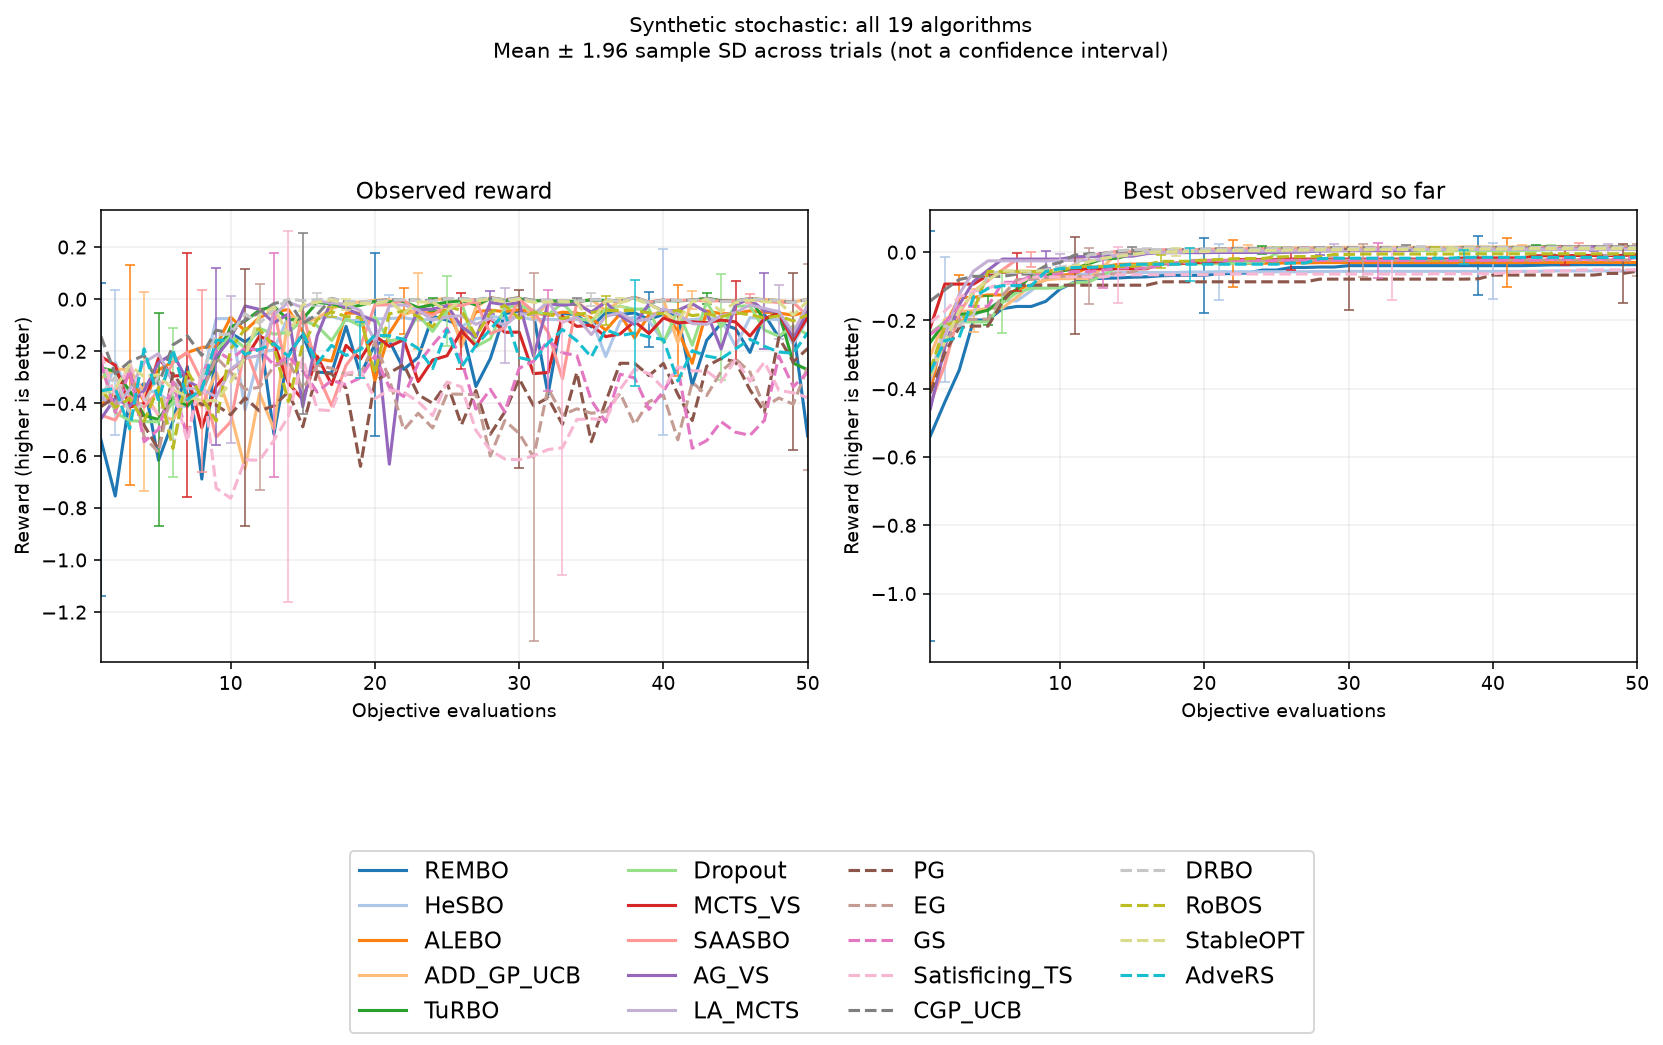
\includegraphics[width=\linewidth,height=.72\textheight,keepaspectratio]{figures/figure-01.png}

{\small\color{BayopyMuted}Captured figure 1 / synthetic stochastic}

\end{center}

\end{minipage}\par\vspace{6pt}

\Needspace{6\baselineskip}
\phantomsection
\subsection*{1.2 Contextual: all algorithms}
\addcontentsline{toc}{subsection}{1.2 Contextual: all algorithms}

\begin{Verbatim}[breaklines=true,breakanywhere=true,fontsize=\small]
    This block defines its own objective, providers, settings, environment,
    and results directory. Every method is reconstructed with explicit
    settings for this environment. Run the complete block independently.\end{Verbatim}


\BlockLabel{Editable Python / block 3}

\CodeFile{code/synthetic_contextual.py}

\BlockLabel{Captured terminal output}

\OutputFile{outputs/synthetic_contextual-01.txt}

\par\noindent\begin{minipage}{\linewidth}

\begin{center}

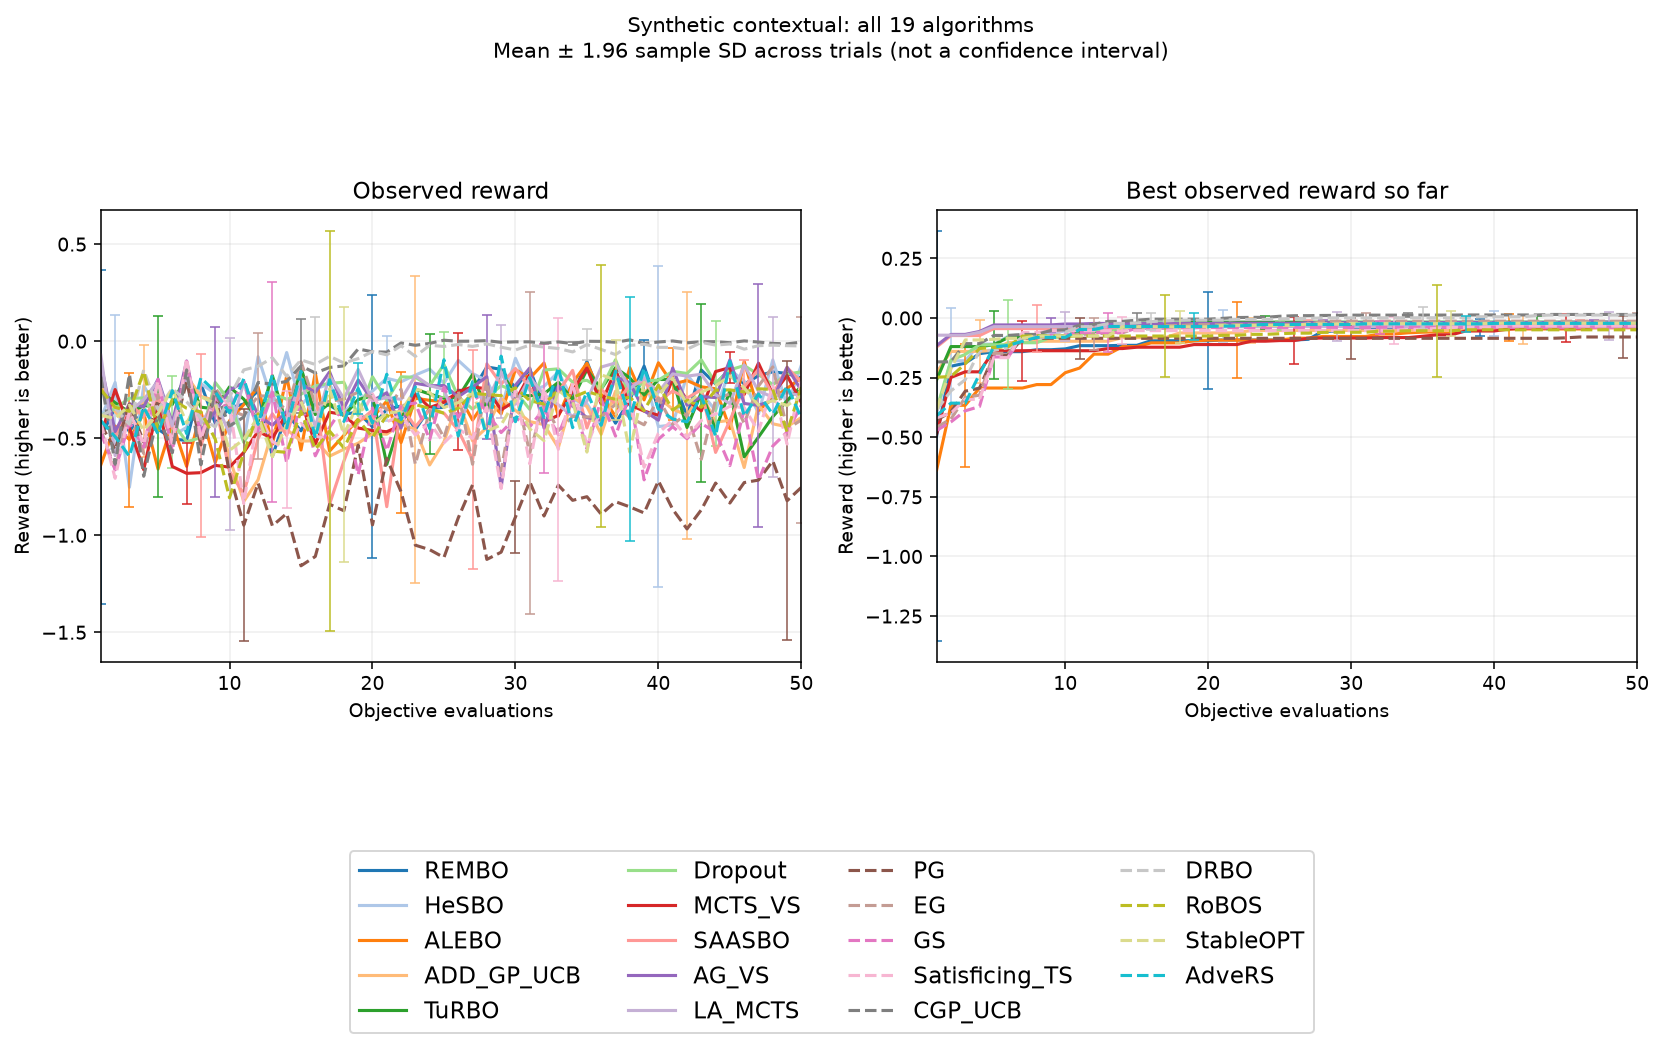
\includegraphics[width=\linewidth,height=.72\textheight,keepaspectratio]{figures/figure-02.png}

{\small\color{BayopyMuted}Captured figure 2 / synthetic contextual}

\end{center}

\end{minipage}\par\vspace{6pt}

\Needspace{6\baselineskip}
\phantomsection
\subsection*{1.3 Distributional: all algorithms}
\addcontentsline{toc}{subsection}{1.3 Distributional: all algorithms}

\begin{Verbatim}[breaklines=true,breakanywhere=true,fontsize=\small]
    This block defines its own objective, providers, settings, environment,
    and results directory. Every method is reconstructed with explicit
    settings for this environment. Run the complete block independently.\end{Verbatim}


\BlockLabel{Editable Python / block 4}

\CodeFile{code/synthetic_distributional.py}

\BlockLabel{Captured terminal output}

\OutputFile{outputs/synthetic_distributional-01.txt}

\par\noindent\begin{minipage}{\linewidth}

\begin{center}

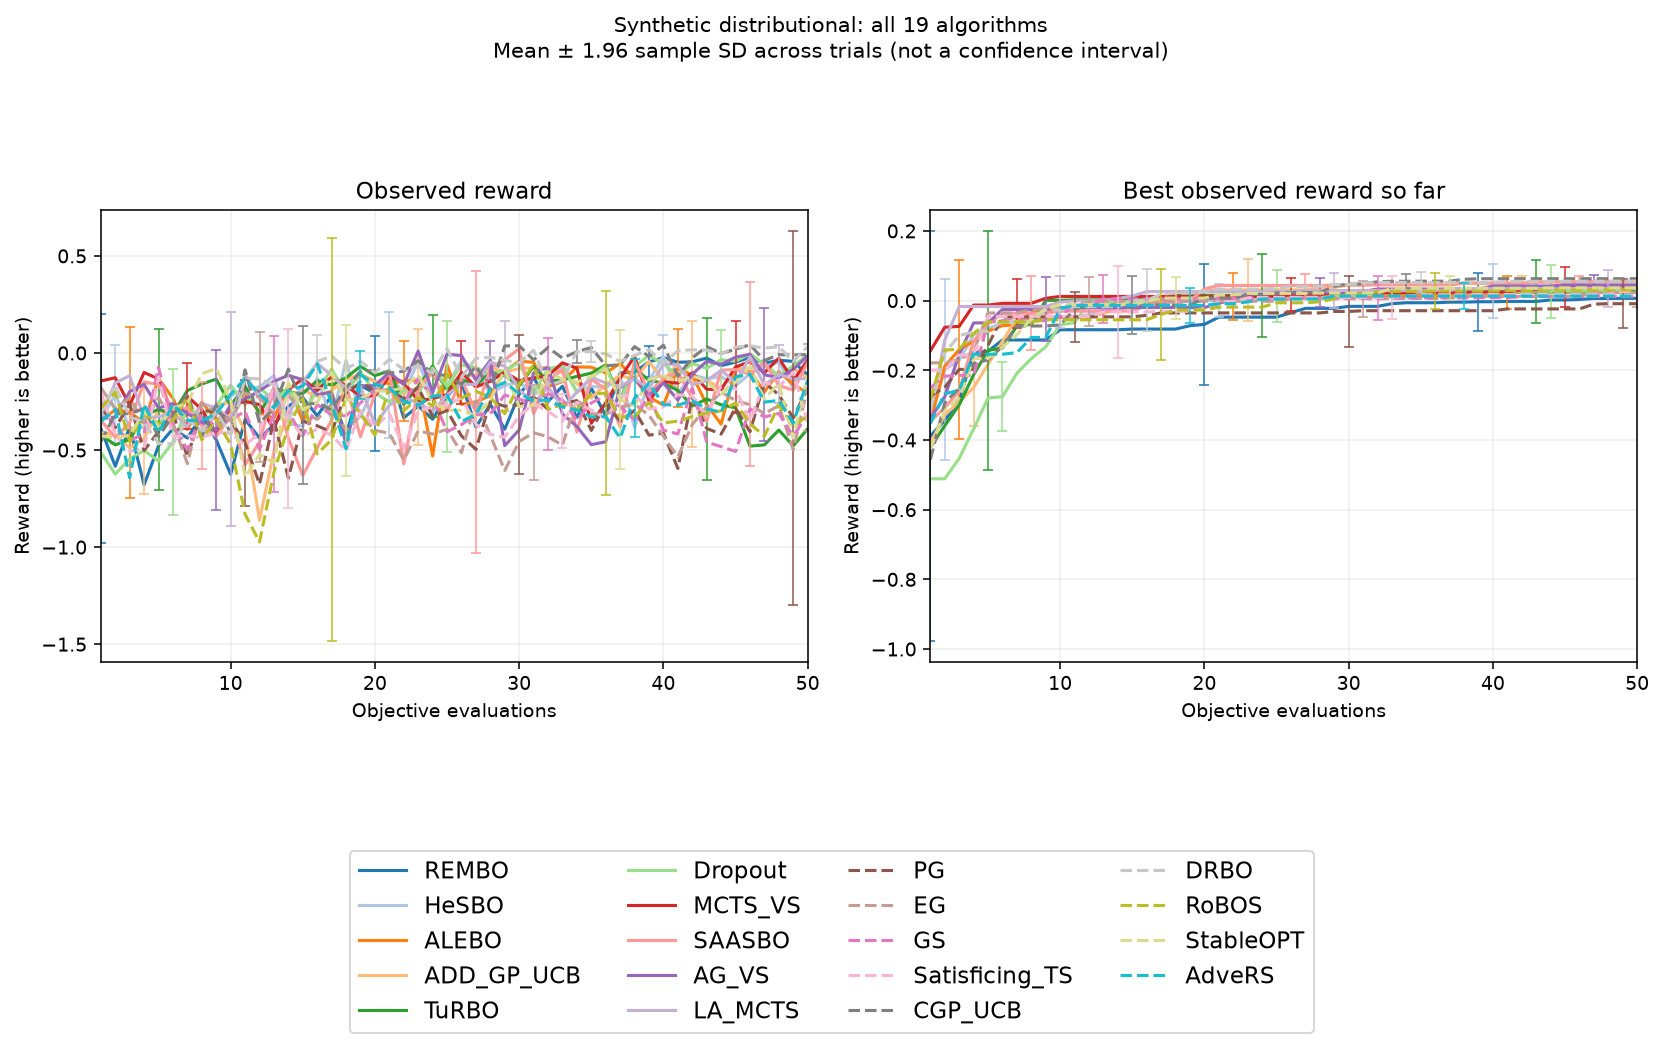
\includegraphics[width=\linewidth,height=.72\textheight,keepaspectratio]{figures/figure-03.png}

{\small\color{BayopyMuted}Captured figure 3 / synthetic distributional}

\end{center}

\end{minipage}\par\vspace{6pt}

\Needspace{6\baselineskip}
\phantomsection
\subsection*{1.4 Adversarial: all algorithms}
\addcontentsline{toc}{subsection}{1.4 Adversarial: all algorithms}

\begin{Verbatim}[breaklines=true,breakanywhere=true,fontsize=\small]
    This block defines its own objective, providers, settings, environment,
    and results directory. Every method is reconstructed with explicit
    settings for this environment. Run the complete block independently.\end{Verbatim}


\BlockLabel{Editable Python / block 5}

\CodeFile{code/synthetic_adversarial.py}

\BlockLabel{Captured terminal output}

\OutputFile{outputs/synthetic_adversarial-01.txt}

\par\noindent\begin{minipage}{\linewidth}

\begin{center}

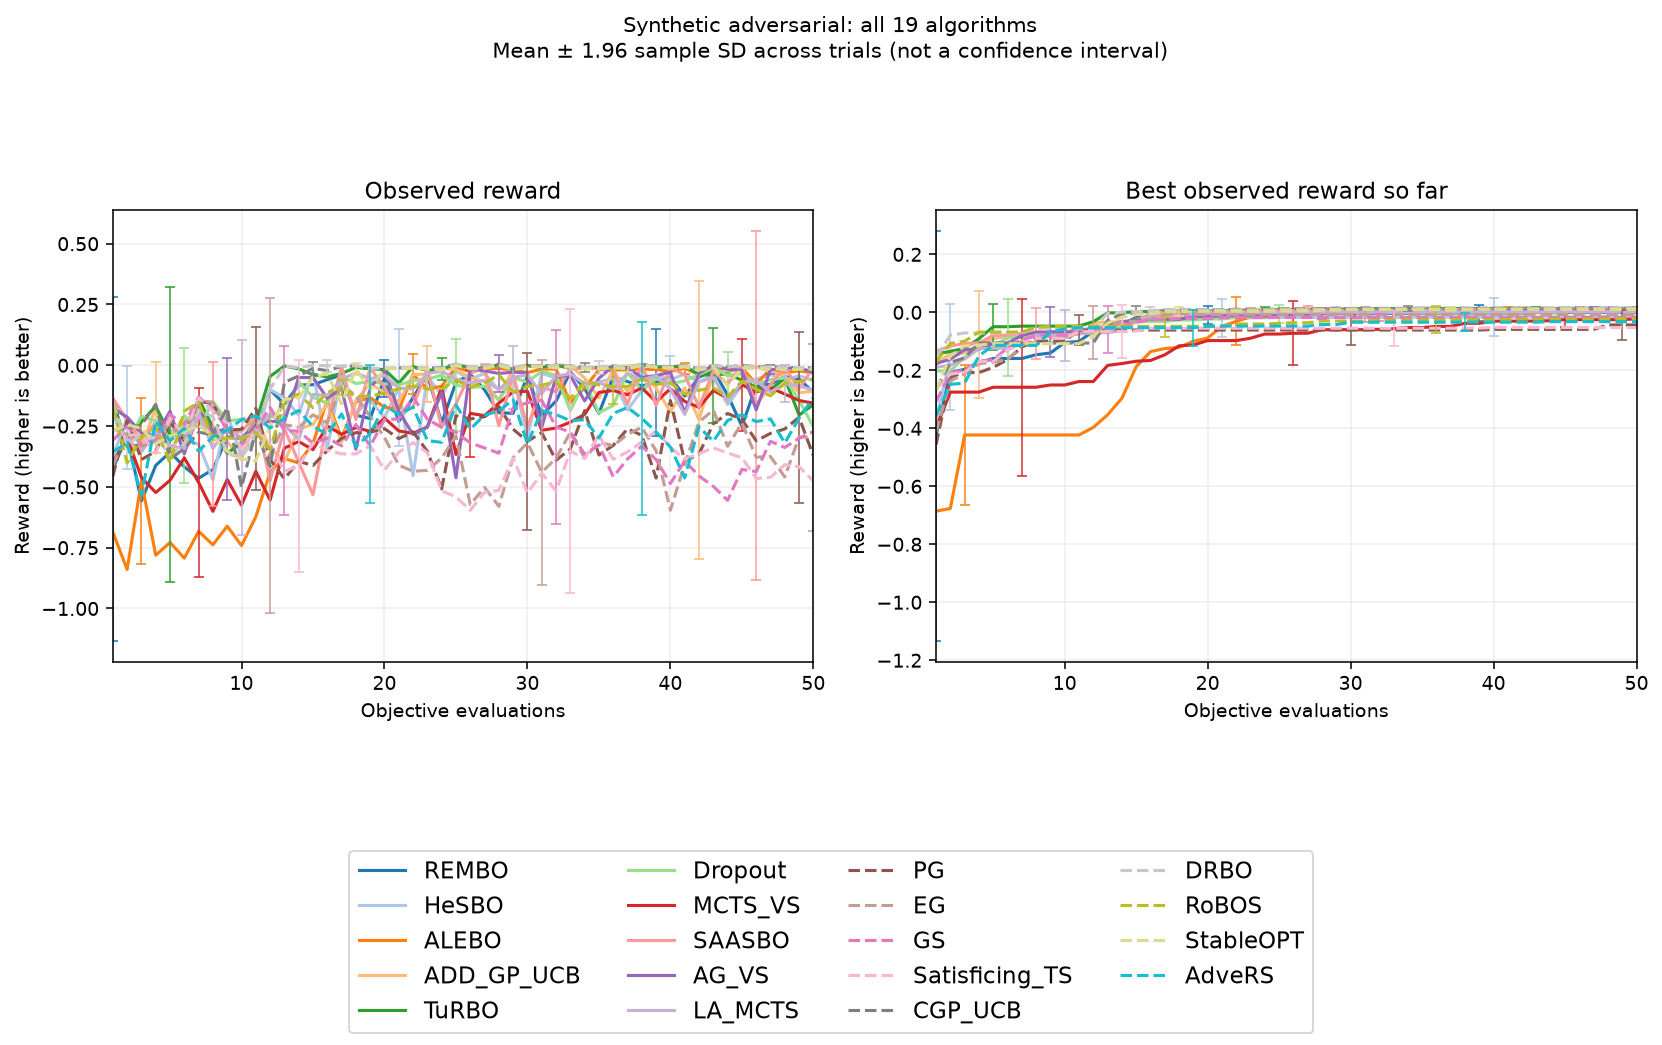
\includegraphics[width=\linewidth,height=.72\textheight,keepaspectratio]{figures/figure-04.png}

{\small\color{BayopyMuted}Captured figure 4 / synthetic adversarial}

\end{center}

\end{minipage}\par\vspace{6pt}

\clearpage
\phantomsection
\section*{2. Real Data Formatting}
\addcontentsline{toc}{section}{2. Real Data Formatting}

The strict native loader is \texttt{bayopy.\allowbreak{}load\_\allowbreak{}dataset(path,\allowbreak{} environment=\allowbreak{}".\allowbreak{}.\allowbreak{}.\allowbreak{}")}. It reads a finite table of \textbf{explicit rewards},\allowbreak{} not a model-training dataset whose last column is an arbitrary label. A row is an observation at the named action and,\allowbreak{} where relevant,\allowbreak{} context. The library never invents missing rewards or interpolates an unmeasured row. Your objective can instead train a model or run a simulator inside a user-defined function if new evaluations are possible.


Reserved columns use zero-based contiguous numbering. \texttt{action\_\allowbreak{}0} through \texttt{action\_\allowbreak{}\{d-1\}} identify learner-controlled coordinates. \texttt{reward} is required and must be the final column. Numeric values must be finite. Context vectors describe exogenous information and need not have the same dimension as actions; there is no automatic one-context-column-per-action-column rule.


{\small
\begin{longtable}{@{}>{\raggedright\arraybackslash}p{0.1800\dimexpr\linewidth-4\tabcolsep\relax}>{\raggedright\arraybackslash}p{0.3500\dimexpr\linewidth-4\tabcolsep\relax}>{\raggedright\arraybackslash}p{0.4700\dimexpr\linewidth-4\tabcolsep\relax}@{}}
\toprule
\textbf{Environment} & \textbf{Required column order / roles} & \textbf{Learner sees before acting} \\
\midrule\endfirsthead
\toprule
\textbf{Environment} & \textbf{Required column order / roles} & \textbf{Learner sees before acting} \\
\midrule\endhead
Stochastic & action\_\allowbreak{}0,\allowbreak{}...,\allowbreak{}action\_\allowbreak{}(d-1),\allowbreak{}reward & Available action coordinates \\
Contextual & action\_\allowbreak{}0,\allowbreak{}...,\allowbreak{}context\_\allowbreak{}0,\allowbreak{}...,\allowbreak{}reward & Current context and actions available there \\
Distributional & action\_\allowbreak{}0,\allowbreak{}...,\allowbreak{}context\_\allowbreak{}0,\allowbreak{}...,\allowbreak{}reference\_\allowbreak{}probability,\allowbreak{} optional sampling\_\allowbreak{}probability and margin,\allowbreak{} reward & Support,\allowbreak{} reference probabilities,\allowbreak{} ambiguity margin \\
Adversarial & action\_\allowbreak{}0,\allowbreak{}...,\allowbreak{}evaluated\_\allowbreak{}action\_\allowbreak{}0,\allowbreak{}...,\allowbreak{}reward & Nominal action coordinates; evaluated coordinate arrives in feedback \\
\bottomrule
\end{longtable}
}

Context is not a reward and must not contain the observed target as a shortcut. Reward columns remain hidden from the learner until the environment evaluates its selected action. This is offline finite search,\allowbreak{} not a causal evaluation of treatments or a policy-value estimator for incomplete logged bandit data. Arbitrary logged actions without counterfactual coverage cannot be treated as a complete distributional reward grid.


The four code blocks below write actual sample rows using only BayOPy,\allowbreak{} reload them,\allowbreak{} and print the exact CSV format. Replace the rows with your own measurements. They demonstrate formatting; the four large experiments use the full external files and reconstruct their own environments.



\Needspace{6\baselineskip}
\phantomsection
\subsection*{Stochastic CSV}
\addcontentsline{toc}{subsection}{Stochastic CSV}

Only action columns and the final reward are required. The example records three scaled patient descriptors and a negative recorded response. Searching rows selects measured records,\allowbreak{} not a medical intervention.



\BlockLabel{Editable Python / block 6}

\CodeFile{code/format_stochastic.py}

\BlockLabel{Captured terminal output}

\OutputFile{outputs/format_stochastic-01.txt}

\Needspace{6\baselineskip}
\phantomsection
\subsection*{Contextual CSV}
\addcontentsline{toc}{subsection}{Contextual CSV}

Context dimensions are independent of action dimensions. Wine cultivar is encoded with three one-hot context columns so numeric distances do not imply an ordering of categories. All action/reward rows at a revealed cultivar are eligible; other cultivars' rewards remain unavailable.



\BlockLabel{Editable Python / block 7}

\CodeFile{code/format_contextual.py}

\BlockLabel{Captured terminal output}

\OutputFile{outputs/format_contextual-01.txt}

\Needspace{6\baselineskip}
\phantomsection
\subsection*{Distributional CSV}
\addcontentsline{toc}{subsection}{Distributional CSV}

Every distinct action must have a measured row at every context in the support. \texttt{reference\_\allowbreak{}probability} must agree across all rows of the same context and sum to one over support,\allowbreak{} not over CSV rows. \texttt{sampling\_\allowbreak{}probability} has the same normalization and is environment-private. When omitted it equals the reference. \texttt{margin} is one consistent non-negative scalar; omitted margin defaults to zero. A multirow CSV repeats this metadata. The wind example uses 11 wind-generation levels. Its rewards are calculated from the published revenue function; they are not measured payments. Include all contexts when writing a smaller example so probabilities still sum to one. The real experiment overrides initial CSV probabilities with chronological 48-hour reference and private realization providers.



\BlockLabel{Editable Python / block 8}

\CodeFile{code/format_distributional.py}

\BlockLabel{Captured terminal output}

\OutputFile{outputs/format_distributional-01.txt}

\Needspace{6\baselineskip}
\phantomsection
\subsection*{Adversarial CSV}
\addcontentsline{toc}{subsection}{Adversarial CSV}

Both nominal and evaluated action vectors have dimension d. The final reward belongs to the evaluated coordinate. This finite-table contract requires a deterministic one-to-one permutation over the measured action set,\allowbreak{} so every attack lookup has a real measured outcome and consumed rows remain consistent. Arbitrary off-grid attacks are rejected in finite mode; use a function-backed environment to evaluate new coordinates. The Iris example constructs swaps between measured records. It is an illustrative adversarial view of observational data,\allowbreak{} not a historical attack dataset.



\BlockLabel{Editable Python / block 9}

\CodeFile{code/format_adversarial.py}

\BlockLabel{Captured terminal output}

\OutputFile{outputs/format_adversarial-01.txt}

\Needspace{6\baselineskip}
\phantomsection
\subsection*{2.1 Real Life Objective Optimization}
\addcontentsline{toc}{subsection}{2.1 Real Life Objective Optimization}

Four \textbf{different} real datasets provide four large independent comparisons. Each submits all 19 algorithms in five trials,\allowbreak{} in stochastic,\allowbreak{} contextual,\allowbreak{} distributional,\allowbreak{} then adversarial order: \textbf{380 submitted algorithm trials}. Non-native combinations use the documented runtime defaults and emit informative warnings. Genuine failures remain visible in summaries and legends. The source's finite reward table is copied privately for each method. No main experiment enables patience,\allowbreak{} target,\allowbreak{} or time stopping; each requests 50 evaluations.


REMBO,\allowbreak{} HeSBO,\allowbreak{} and ALEBO use \texttt{finite\_\allowbreak{}candidate\_\allowbreak{}mode=\allowbreak{}"project"} by default. This explicit finite-data extension compresses normalized candidate rows: REMBO uses least-squares coordinates,\allowbreak{} HeSBO uses signed bucket averages (zero for empty buckets),\allowbreak{} and ALEBO uses its B projection. Acquisition scores select an actual available row and the environment returns its stored reward. The wind table stores explicitly modeled revenue; its physical context comes from measurements. No reward interpolation is performed by the library. Projection can merge distinct rows,\allowbreak{} so the original embedding guarantees do not apply. The warning \texttt{data.\allowbreak{}projected\_\allowbreak{}embedding} explains this adaptation. Set the configuration field to \texttt{"exact"} to restore strict embedding checks.


The original environment classes remain in use. Context still restricts available contextual rows,\allowbreak{} the distribution still selects the wind-generation context,\allowbreak{} and the adversarial environment still applies its declared attack. These stochastic policies model pooled scalar feedback without conditioning on those additional inputs; execution does not imply contextual or robust optimality. A distribution alone is not enough: evaluation still requires a reward table or callable objective.


{\small
\begin{longtable}{@{}>{\raggedright\arraybackslash}p{0.1800\dimexpr\linewidth-4\tabcolsep\relax}>{\raggedright\arraybackslash}p{0.3500\dimexpr\linewidth-4\tabcolsep\relax}>{\raggedright\arraybackslash}p{0.4700\dimexpr\linewidth-4\tabcolsep\relax}@{}}
\toprule
\textbf{Environment} & \textbf{Distinct external dataset} & \textbf{Reward and constructed interpretation} \\
\midrule\endfirsthead
\toprule
\textbf{Environment} & \textbf{Distinct external dataset} & \textbf{Reward and constructed interpretation} \\
\midrule\endhead
Stochastic & Diabetes & Negative recorded one-year progression; search among measured descriptor rows \\
Contextual & Wine & Recorded proline concentration,\allowbreak{} conditional on one-hot cultivar \\
Distributional & OPSD German wind generation (2013) & Energy commitment revenue under recorded wind realizations; modeled revenue,\allowbreak{} not measured market payments \\
Adversarial & Iris & Measured sepal length at a permuted observed coordinate \\
\bottomrule
\end{longtable}
}

These are explicitly constructed finite optimization views of four real observational tables. They were not collected as four native online bandit trials. The results do not establish clinical benefits,\allowbreak{} causal effects,\allowbreak{} distributional robustness,\allowbreak{} or adversarial guarantees for the original studies. We optimize the stated scalar rewards,\allowbreak{} including the explicit wind revenue model,\allowbreak{} not classification accuracy. For your own application,\allowbreak{} select a reward whose maximization is meaningful.


Provenance,\allowbreak{} source URLs,\allowbreak{} exact transformations,\allowbreak{} and SHA-256 hashes are in \texttt{data/\allowbreak{}native\_\allowbreak{}manifest.\allowbreak{}json}. The original files and prepared CSVs remain under the project-level \texttt{data/\allowbreak{}} folder; none are packaged inside BayOPy. Dataset descriptions are documented by \href{https://scikit-learn.org/1.6/datasets/toy_dataset.html}{scikit-learn's dataset reference} and the wind-source and DRBO references in the distributional subsection.


In the adversarial Iris experiment,\allowbreak{} StableOPT's selected radius 2 covers the entire [0,\allowbreak{}1]\textasciicircum{}3 action box and the constructed swaps. AdveRS instead considers the full feasible domain without receiving the environment's actual attack budget. A small-radius assumption would be false for these data. Best observed reward traces measure sampled outcomes,\allowbreak{} not the robust objectives optimized by DRBO,\allowbreak{} RoBOS,\allowbreak{} StableOPT,\allowbreak{} or AdveRS.



\Needspace{6\baselineskip}
\phantomsection
\subsubsection*{Stochastic: diabetes / all 19 algorithms}
\addcontentsline{toc}{subsubsection}{Stochastic: diabetes / all 19 algorithms}

Run this entire block independently. Its CSV path,\allowbreak{} full algorithm configurations,\allowbreak{} and environment are declared again here.



\BlockLabel{Editable Python / block 10}

\CodeFile{code/real_stochastic.py}

\BlockLabel{Captured terminal output}

\OutputFile{outputs/real_stochastic-01.txt}

\par\noindent\begin{minipage}{\linewidth}

\begin{center}

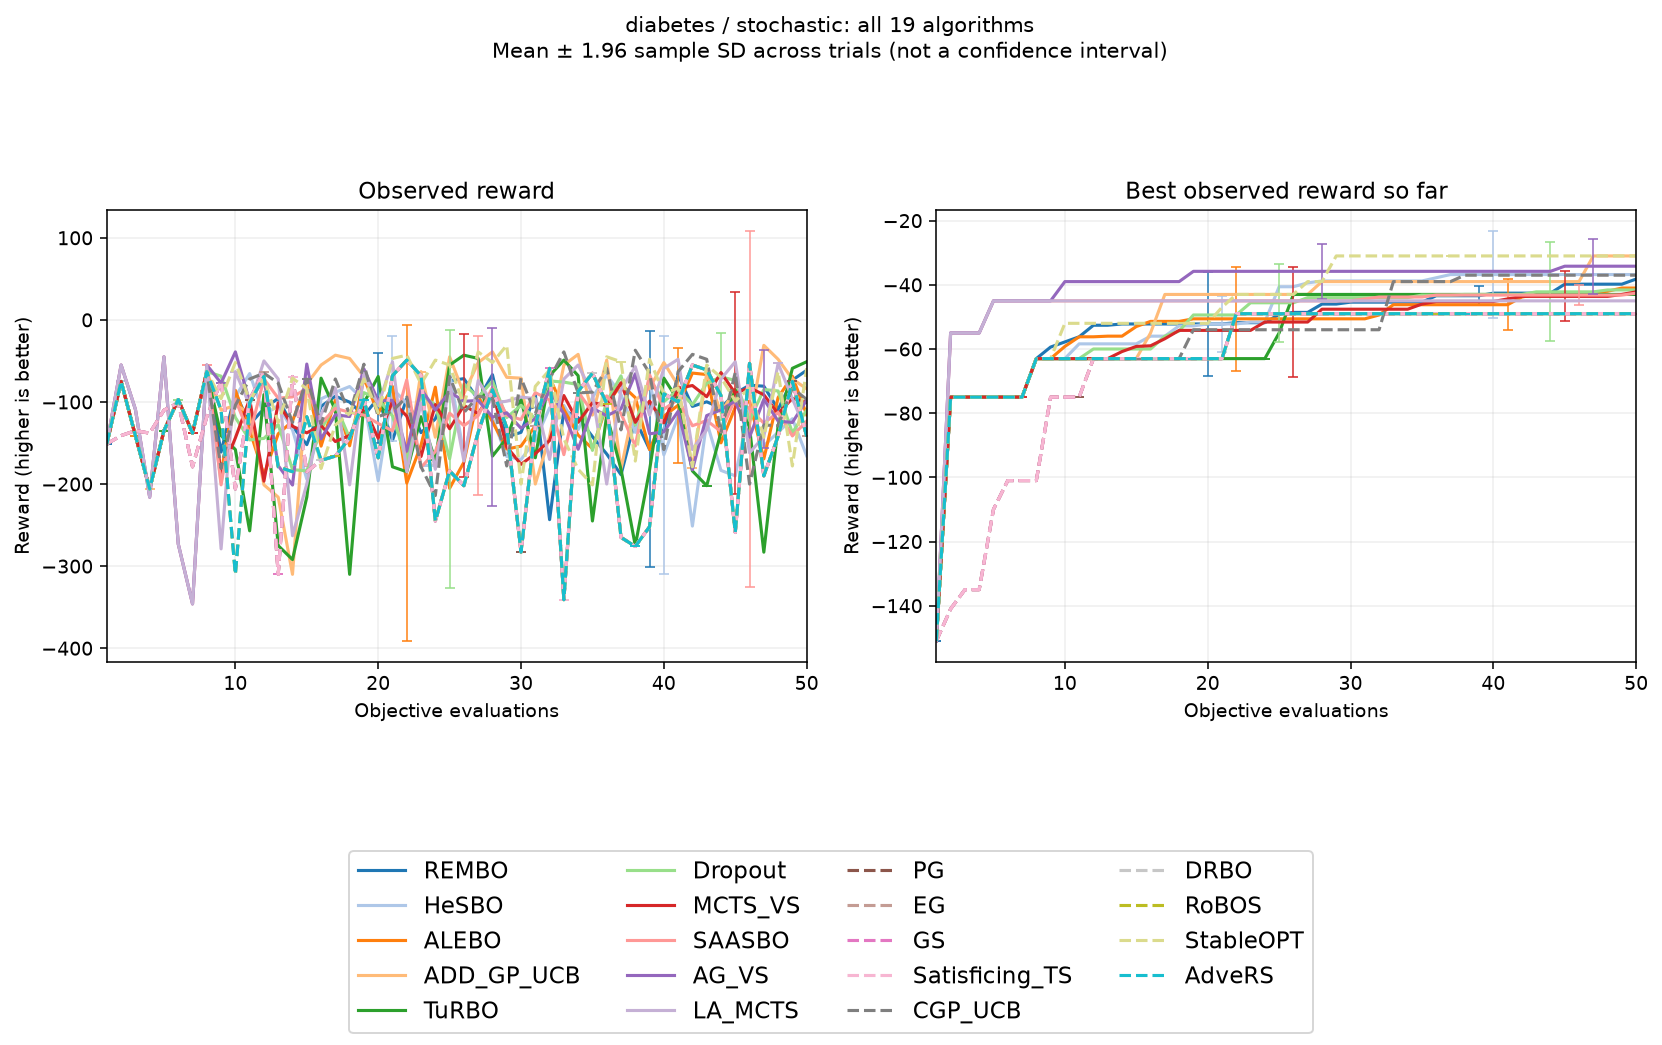
\includegraphics[width=\linewidth,height=.72\textheight,keepaspectratio]{figures/figure-05.png}

{\small\color{BayopyMuted}Captured figure 5 / real stochastic}

\end{center}

\end{minipage}\par\vspace{6pt}

\Needspace{6\baselineskip}
\phantomsection
\subsubsection*{Contextual: wine / all 19 algorithms}
\addcontentsline{toc}{subsubsection}{Contextual: wine / all 19 algorithms}

Run this entire block independently. Its CSV path,\allowbreak{} full algorithm configurations,\allowbreak{} and environment are declared again here.



\BlockLabel{Editable Python / block 11}

\CodeFile{code/real_contextual.py}

\BlockLabel{Captured terminal output}

\OutputFile{outputs/real_contextual-01.txt}

\par\noindent\begin{minipage}{\linewidth}

\begin{center}

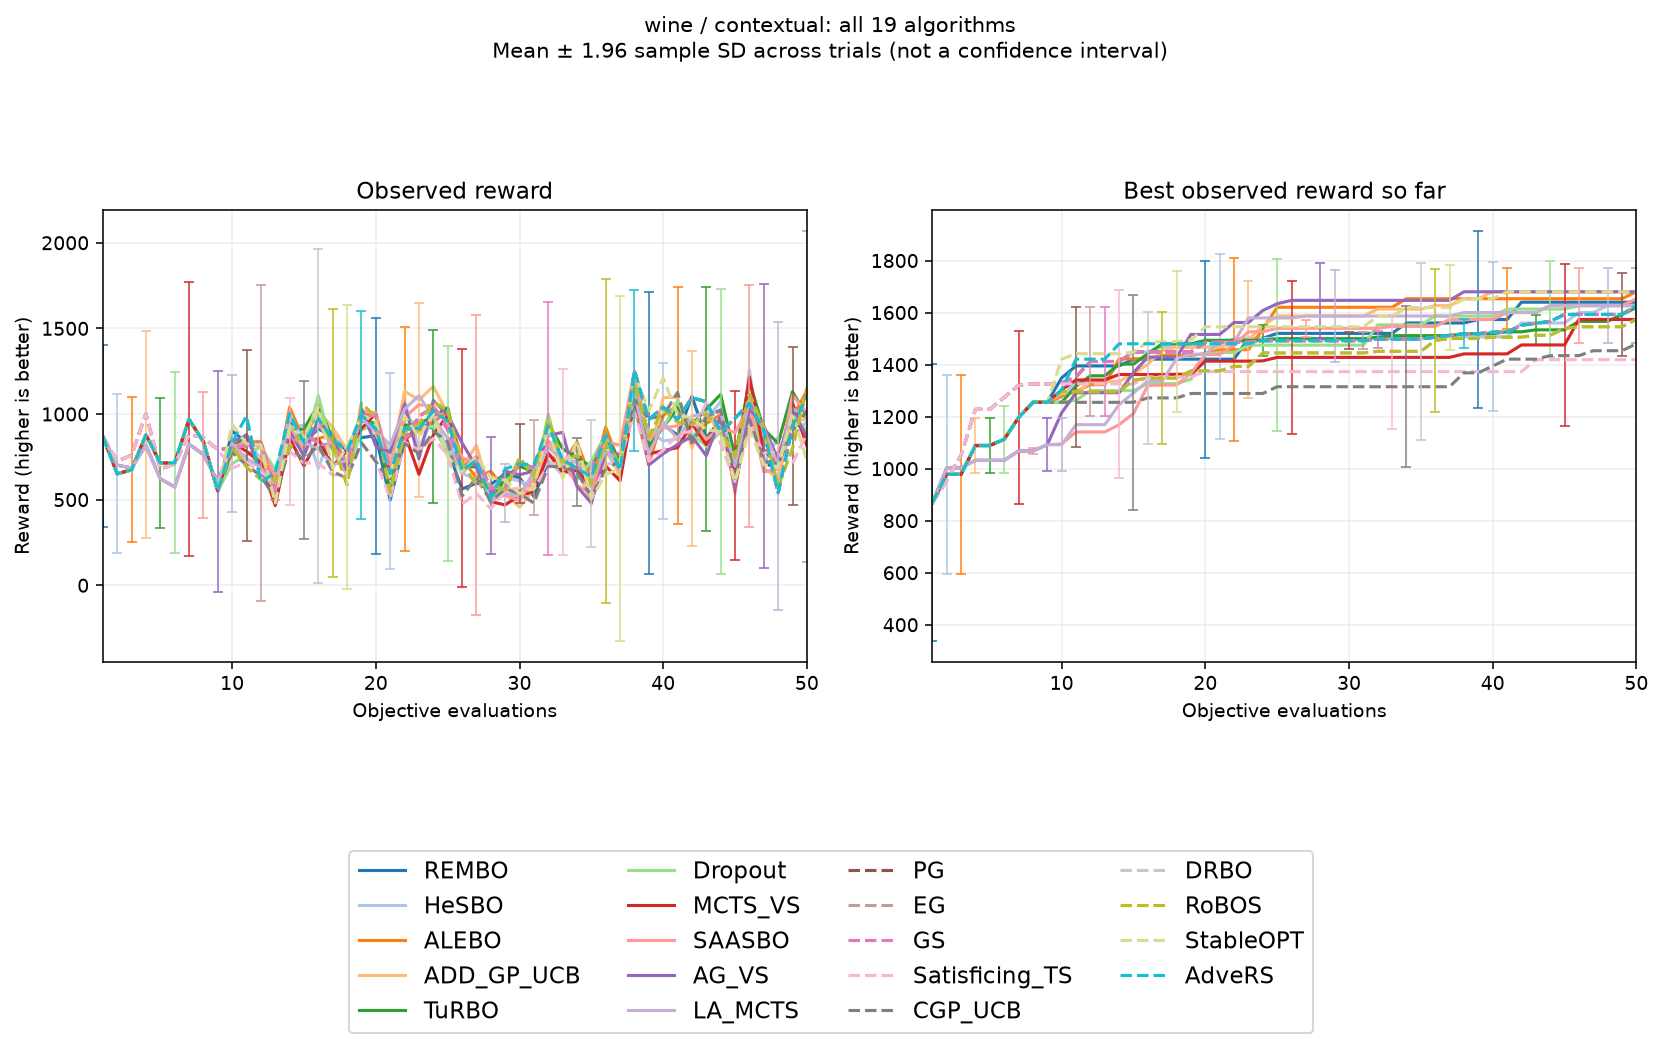
\includegraphics[width=\linewidth,height=.72\textheight,keepaspectratio]{figures/figure-06.png}

{\small\color{BayopyMuted}Captured figure 6 / real contextual}

\end{center}

\end{minipage}\par\vspace{6pt}

\Needspace{6\baselineskip}
\phantomsection
\subsubsection*{Distributional: wind\_\allowbreak{}power / all 19 algorithms}
\addcontentsline{toc}{subsubsection}{Distributional: wind\_\allowbreak{}power / all 19 algorithms}

Run this entire block independently. Its CSV path,\allowbreak{} full algorithm configurations,\allowbreak{} and environment are declared again here.



\Needspace{6\baselineskip}
\phantomsection
\subsubsection*{Distributional wind-power commitment: dataset and replay}
\addcontentsline{toc}{subsubsection}{Distributional wind-power commitment: dataset and replay}

This replaces the breast-cancer example with hourly wind-generation data from \href{https://data.open-power-system-data.org/time_series/2019-06-05/}{Open Power System Data,\allowbreak{} version 2019-06-05},\allowbreak{} the data package cited in \href{https://proceedings.mlr.press/v108/kirschner20a/kirschner20a.pdf}{DRBO,\allowbreak{} Section 4}. The retained source contains 98 consecutive German hourly observations from January 2013: generation,\allowbreak{} capacity,\allowbreak{} and capacity factor.


The action is promised energy as a fraction of capacity; context is realized wind generation. The paper's revenue is \texttt{0.1*max(c-x,\allowbreak{} 0) + min(x,\allowbreak{}c) - 5*max(x-c,\allowbreak{} 0)}. Here,\allowbreak{} a complete CSV table evaluates that formula on 101 action values and 11 context values. These revenues are calculated from an economic model; they are not recorded electricity payments.


The guide replays 50 consecutive hours after an initial 48-hour history,\allowbreak{} rounding recorded capacity factors to the nearest 0.1. Each round's public reference uses only its preceding 48 observations. The environment's private sampling distribution puts probability one on that hour's recorded,\allowbreak{} quantized realization; future context is not passed to the algorithm. The fixed ambiguity margin 0.1 is illustrative,\allowbreak{} not calibrated to guarantee coverage. Repeated commitments are allowed. All 19 methods receive the same chronological trace,\allowbreak{} with 5 independent algorithm seeds and at most 50 evaluations each.


This small replay is an adaptation of the paper's application,\allowbreak{} not a reproduction of its annual simulator experiment or robust-regret figures. The plotted observed reward and best-observed reward do not measure robust regret; a lucky high-wind hour can improve the latter. Because the physical action is one-dimensional,\allowbreak{} embedding dimension is also one; this example does not demonstrate an advantage from high-dimensional embedding.


RoBOS uses a Matern-3/2 context kernel to avoid the initially configured RBF kernel's near-singular Gram matrix on this support. Completed trials of the other 18 methods were resumed unchanged; RoBOS was rerun.



\BlockLabel{Editable Python / block 12}

\CodeFile{code/real_distributional.py}

\BlockLabel{Captured terminal output}

\OutputFile{outputs/real_distributional-01.txt}

\par\noindent\begin{minipage}{\linewidth}

\begin{center}

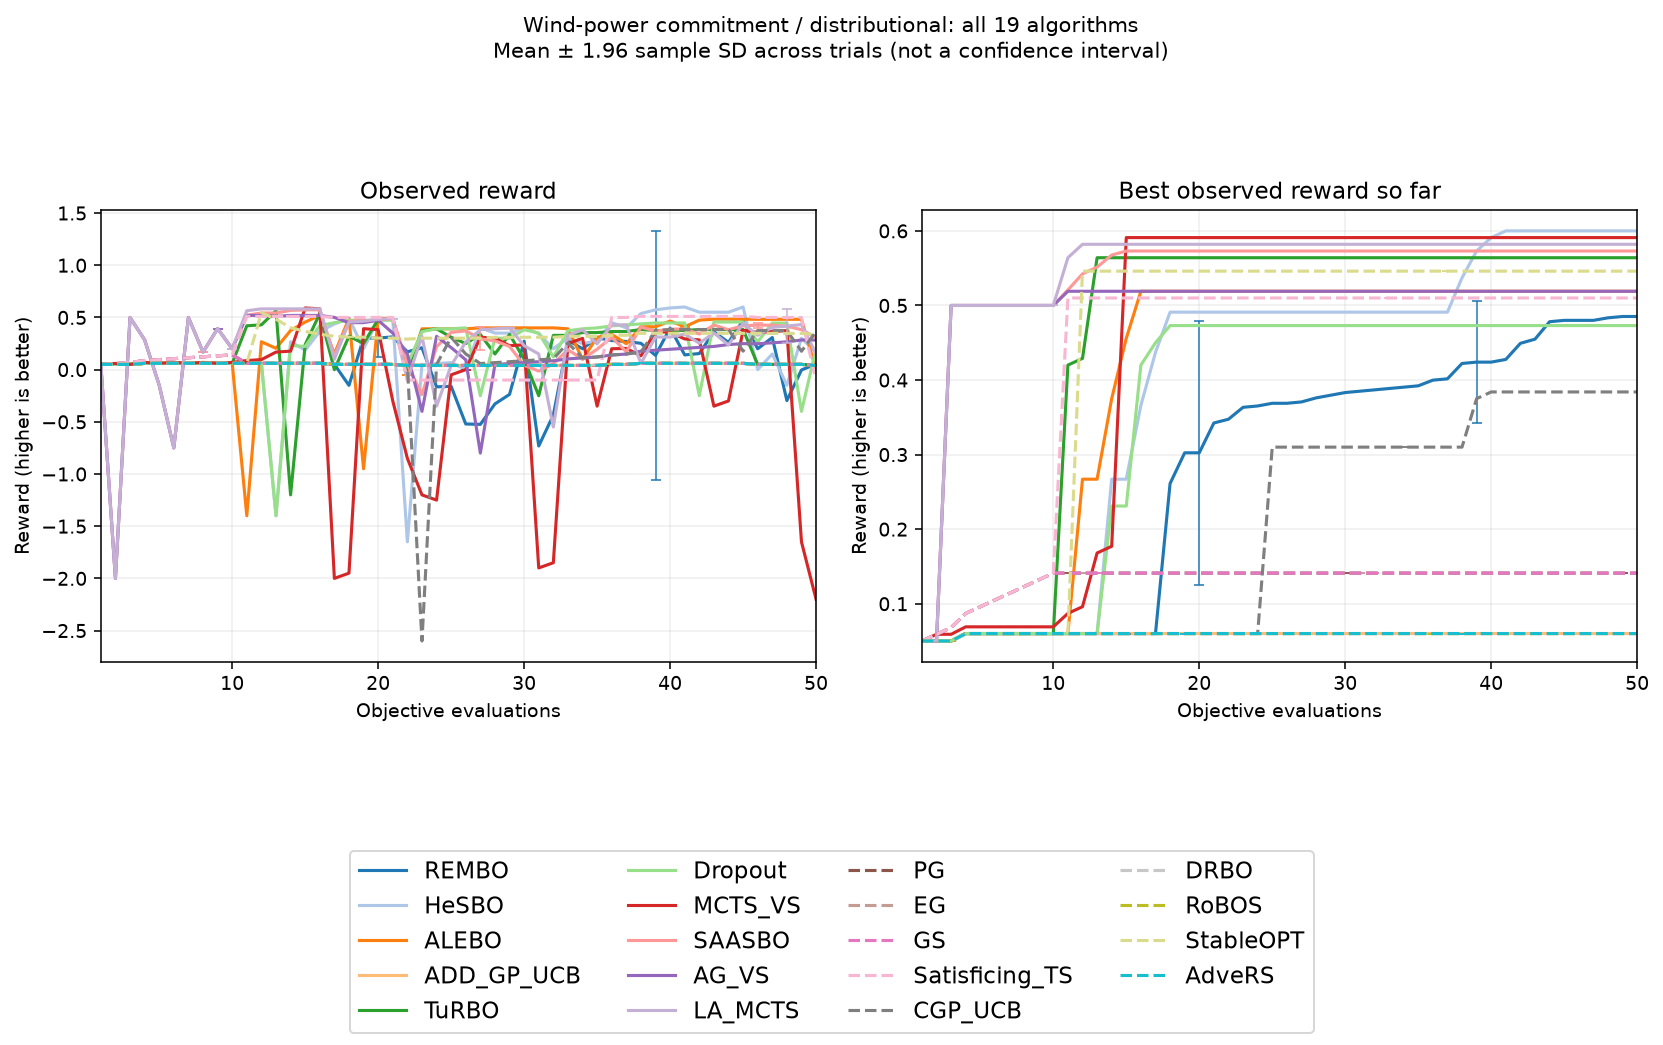
\includegraphics[width=\linewidth,height=.72\textheight,keepaspectratio]{figures/figure-07.png}

{\small\color{BayopyMuted}Captured figure 7 / real distributional}

\end{center}

\end{minipage}\par\vspace{6pt}

\Needspace{6\baselineskip}
\phantomsection
\subsubsection*{Adversarial: iris / all 19 algorithms}
\addcontentsline{toc}{subsubsection}{Adversarial: iris / all 19 algorithms}

Run this entire block independently. Its CSV path,\allowbreak{} full algorithm configurations,\allowbreak{} and environment are declared again here.



\BlockLabel{Editable Python / block 13}

\CodeFile{code/real_adversarial.py}

\BlockLabel{Captured terminal output}

\OutputFile{outputs/real_adversarial-01.txt}

\par\noindent\begin{minipage}{\linewidth}

\begin{center}

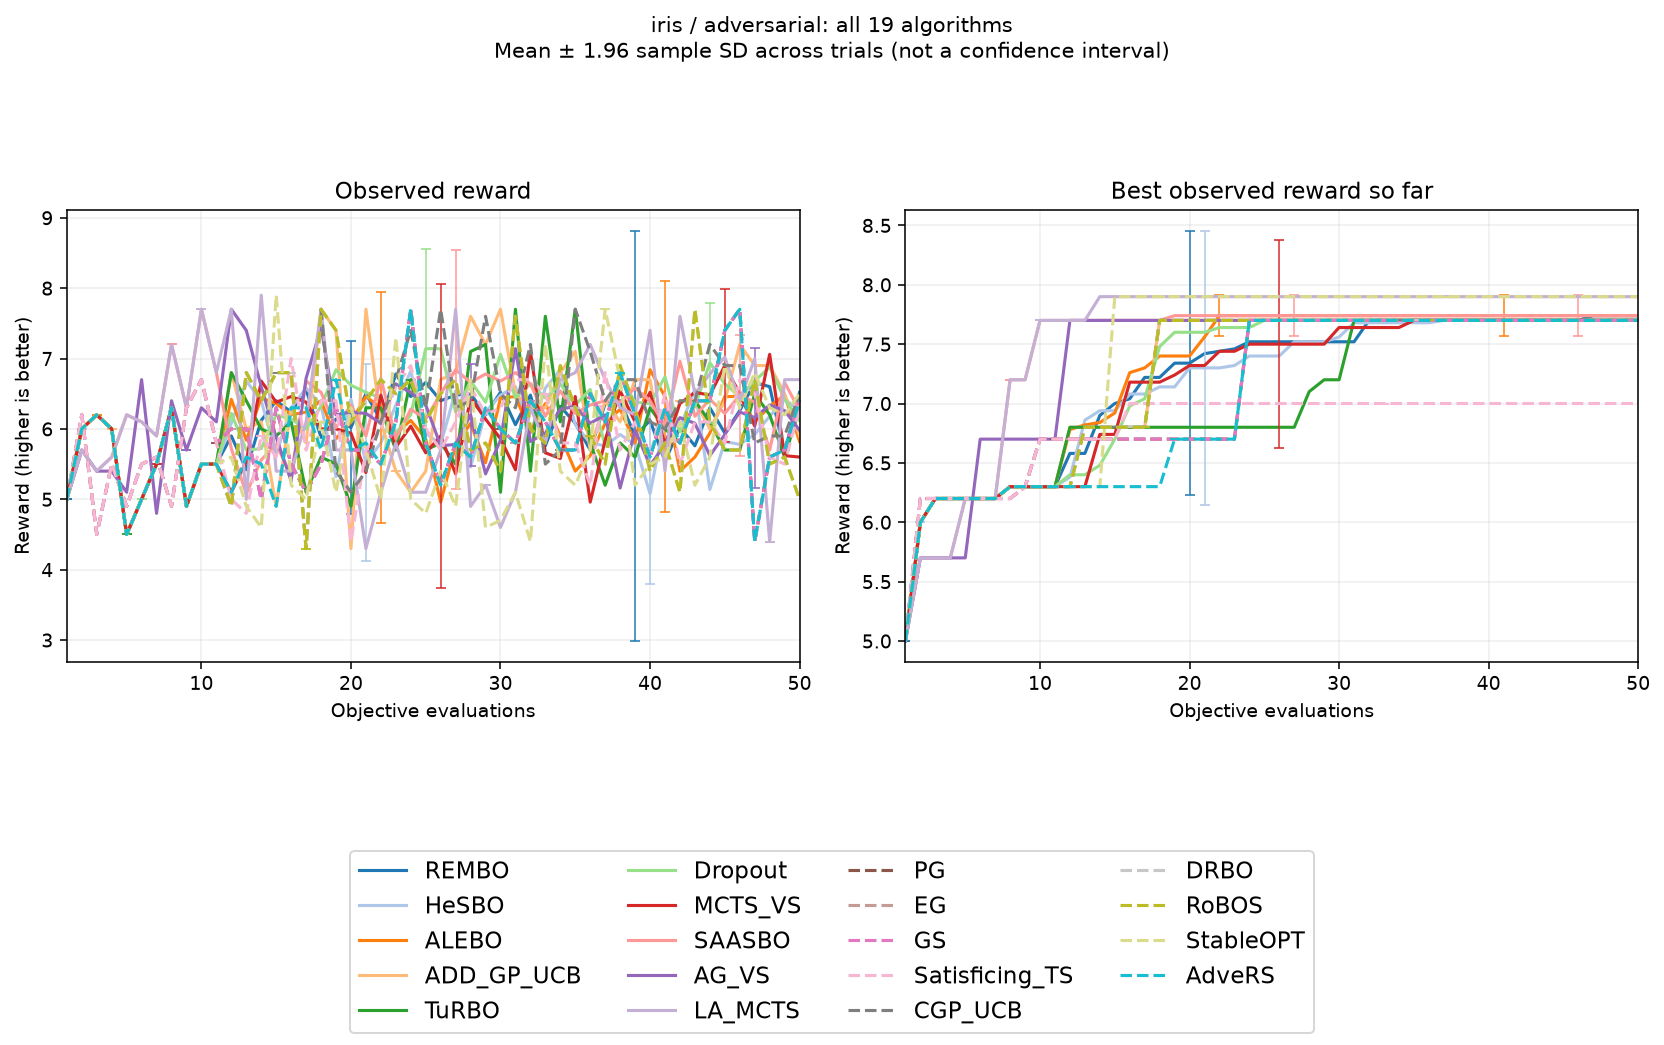
\includegraphics[width=\linewidth,height=.72\textheight,keepaspectratio]{figures/figure-08.png}

{\small\color{BayopyMuted}Captured figure 8 / real adversarial}

\end{center}

\end{minipage}\par\vspace{6pt}

\clearpage
\phantomsection
\section*{3. Early Stopping}
\addcontentsline{toc}{section}{3. Early Stopping}

The eight preceding main comparisons used only a 50-evaluation cap. Here we explicitly enable other stopping mechanisms. \texttt{make\_\allowbreak{}stopping()} returns fresh rule instances because patience tracks history. A multi-algorithm Experiment clones the supplied rule for each child; progress in one method cannot stop another. Each example below is independent.


{\small
\begin{longtable}{@{}>{\raggedright\arraybackslash}p{0.5000\dimexpr\linewidth-2\tabcolsep\relax}>{\raggedright\arraybackslash}p{0.5000\dimexpr\linewidth-2\tabcolsep\relax}@{}}
\toprule
\textbf{Rule} & \textbf{Meaning} \\
\midrule\endfirsthead
\toprule
\textbf{Rule} & \textbf{Meaning} \\
\midrule\endhead
MaximumEvaluationsStoppingRule & Stop after the allowed number of evaluated actions,\allowbreak{} counting initialization \\
MaximumRoundsStoppingRule & Limit ask/tell rounds; a batch can contain several evaluations \\
MaximumTimeStoppingRule & Check elapsed time between complete rounds; does not interrupt an optimizer \\
TargetValueStoppingRule & Stop when the best observed reward reaches a target \\
NoImprovementStoppingRule & Stop after patience rounds without improvement exceeding min\_\allowbreak{}delta,\allowbreak{} after min\_\allowbreak{}rounds \\
any\_\allowbreak{}of / all\_\allowbreak{}of & Compose conditions; any condition versus every condition \\
\bottomrule
\end{longtable}
}

\texttt{run(max\_\allowbreak{}evaluations=\allowbreak{}50)} remains a separate hard safety cap. If a full batch would exceed the remaining budget,\allowbreak{} the runner stops before that batch rather than changing its acquisition semantics. For batch size 3,\allowbreak{} a cap of 50 can therefore end at 48 evaluations. Rule checks occur at completed-round boundaries. No-improvement and target rules concern observed rewards; noise can trigger them without finding the latent optimum. Method-specific posterior stopping is separate: AG\_\allowbreak{}VS accepts \texttt{stopping\_\allowbreak{}threshold} and \texttt{stopping\_\allowbreak{}delta} together; leaving both as None disables it. Its \texttt{stagnation\_\allowbreak{}patience} causes internal reinitialization,\allowbreak{} not experiment termination.



\BlockLabel{Editable Python / block 14}

\CodeFile{code/early_patience.py}

\BlockLabel{Captured terminal output}

\OutputFile{outputs/early_patience-01.txt}

\par\noindent\begin{minipage}{\linewidth}

\begin{center}

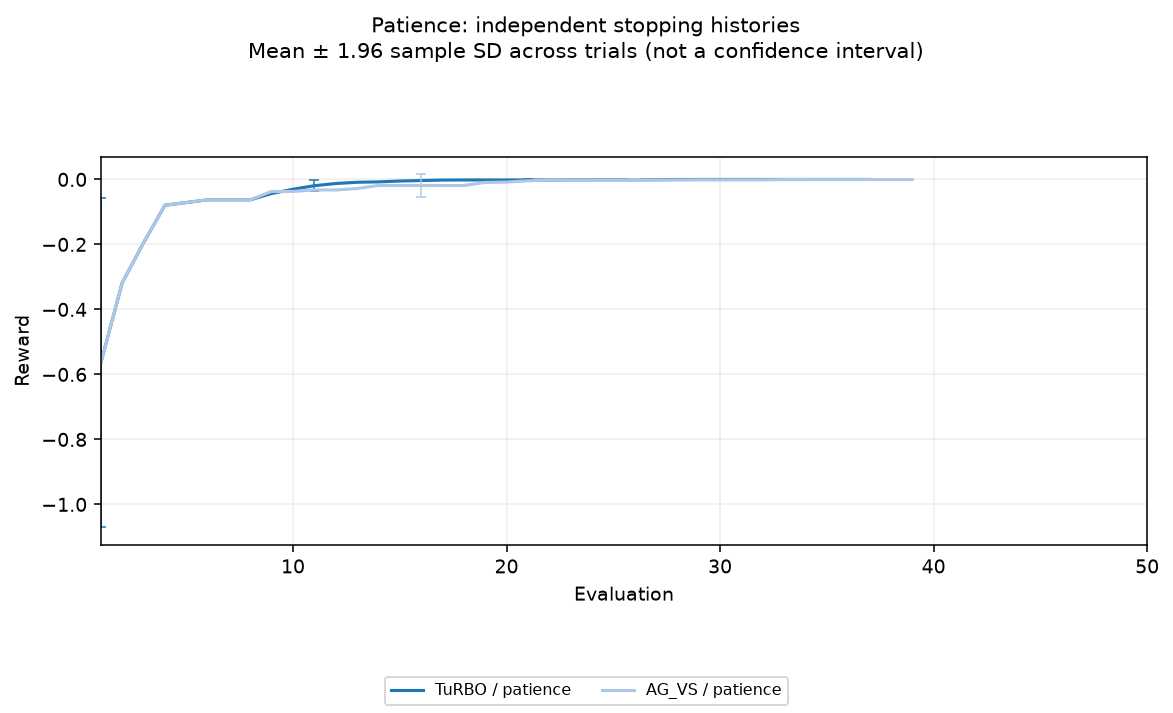
\includegraphics[width=\linewidth,height=.72\textheight,keepaspectratio]{figures/figure-09.png}

{\small\color{BayopyMuted}Captured figure 9 / early patience}

\end{center}

\end{minipage}\par\vspace{6pt}

\BlockLabel{Editable Python / block 15}

\CodeFile{code/early_composition.py}

\BlockLabel{Captured terminal output}

\OutputFile{outputs/early_composition-01.txt}

\par\noindent\begin{minipage}{\linewidth}

\begin{center}

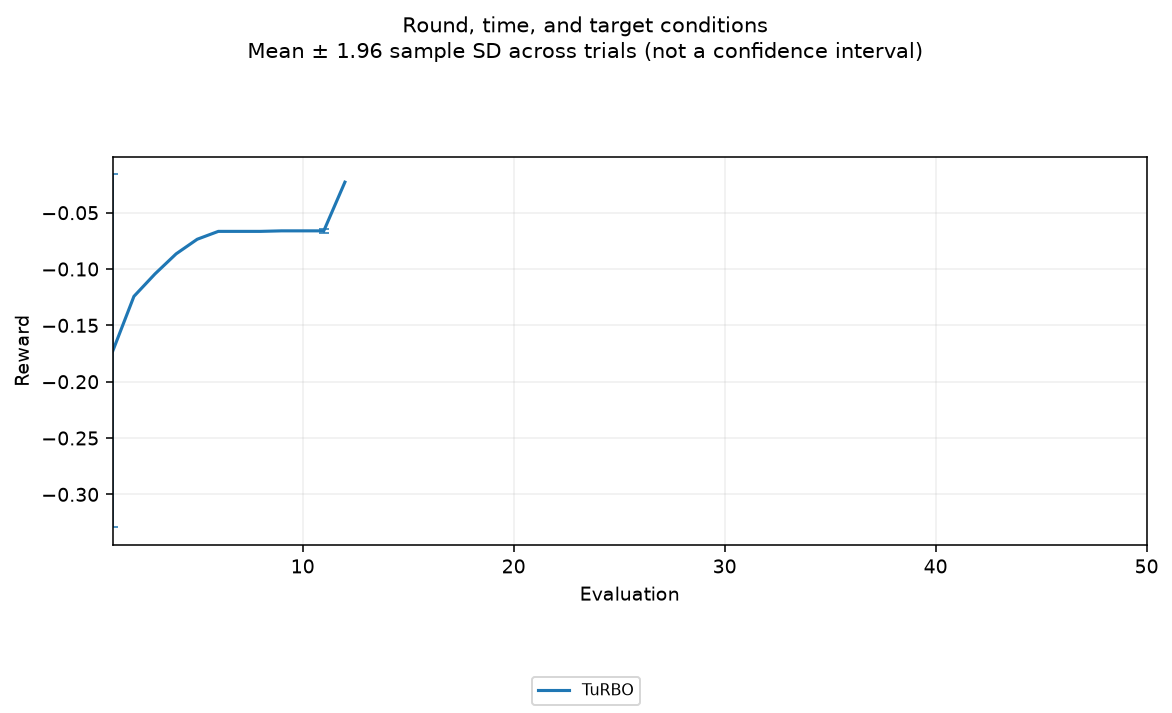
\includegraphics[width=\linewidth,height=.72\textheight,keepaspectratio]{figures/figure-10.png}

{\small\color{BayopyMuted}Captured figure 10 / early composition}

\end{center}

\end{minipage}\par\vspace{6pt}

\Needspace{6\baselineskip}
\phantomsection
\subsection*{Accuracy and interpretation of the measured results}
\addcontentsline{toc}{subsection}{Accuracy and interpretation of the measured results}

Every large experiment reports warnings,\allowbreak{} failed contracts,\allowbreak{} actual evaluation counts,\allowbreak{} and captured output. A common best-observed-reward trace is useful for inspecting execution; it is not the same as every method's mathematical objective. Contextual rewards depend on context. DRBO optimizes a worst-case distributional value; StableOPT uses robust confidence bounds. A high noisy observation alone does not establish robustness or global convergence.


Internal zero-context,\allowbreak{} point-mass-distribution and zero-perturbation defaults are interoperability extensions. The original papers do not claim that these choices recover native contextual,\allowbreak{} distributional or adversarial performance in every environment. The environment still owns action evaluation and reward feedback. Warnings identify the assumptions changed for execution; a curve obtained under an adaptation must be interpreted under that adaptation.


The numerical audit found and fixed a DRBO local-search defect: an accepted solver endpoint could be worse than the already-scored start,\allowbreak{} and flat surfaces could make Powell drift toward a boundary. After successful solver certification,\allowbreak{} the implementation now re-certifies and retains the start unless refinement improves it beyond tolerance. All-failed solver cases still raise. Focused tests cover worse endpoints,\allowbreak{} plateaus,\allowbreak{} and certification.


ALEBO's constrained acquisition optimizer could reject every local endpoint despite having usable feasible candidates. A reproduced failure after 43 evaluations had SLSQP reporting success with constraint residuals of 3.24e-9 and 2.18e-7,\allowbreak{} above the configured 1e-9 feasibility tolerance. It now screens the feasible candidate pool,\allowbreak{} refines its best starts with analytic gradients when available,\allowbreak{} and independently verifies each endpoint. It retains the best finite feasible candidate when refinement cannot improve it; refinement diagnostics remain visible as warnings. Feasible screening and constrained gradient refinement follow the \href{https://github.com/facebook/Ax/blob/0.1.17/ax/models/torch/alebo.py#L470-L526}{official Ax ALEBO acquisition optimizer} and the \href{https://proceedings.neurips.cc/paper_files/paper/2020/file/10fb6cfa4c990d2bad5ddef4f70e8ba2-Paper.pdf}{paper's constrained search domain}. The correction preserves the polytope and metric-inference model; it does not relax feasibility or establish global acquisition optimality. Targeted tests cover infeasible and worse local endpoints. The failing checkpoint subsequently continued to 50 evaluations,\allowbreak{} and a fresh five-trial check completed all five 50-evaluation runs with feasible actions.


This ALEBO correction concerns acquisition search only. The existing option named \texttt{metric\_\allowbreak{}inference=\allowbreak{}"laplace"} records fixed-scale Gaussian perturbations of fitted lower-factor parameters; it does not derive a Laplace covariance from the posterior Hessian. Acquisition decisions still use the fitted GP,\allowbreak{} rather than averaging over those recorded metric samples. The displayed results therefore do not establish equivalence to the paper's integrated metric inference. That separate modeling limitation remains explicit.


Checkpoint checks compare resumed actions and rewards with uninterrupted runs,\allowbreak{} including independent trial random states and an interruption after an environment measurement was committed but before algorithm feedback. Restoring the GoodAction family's GP warm start and fitting cadence prevents continuation from silently following a different numerical path. Immutable setting mismatches and corrupt checkpoints are rejected before replacing saved aggregate results. These checks concern BayOPy's state; external simulators and side-effecting objectives need their own durable state.


A separate bounded resume audit covered all 19 methods in their native environments with two seeds each. It checkpointed after each method's initial design (8-11 evaluations) and continued through two model-based choices: resumed actions and rewards matched uninterrupted runs exactly in this audit. Its records are retained in \texttt{results/\allowbreak{}resume\_\allowbreak{}catalog/\allowbreak{}validation.\allowbreak{}json}. This small continuation check complements the five-trial guide experiments; it is not a claim of exact reproducibility across every device,\allowbreak{} dependency version or external system.


The frozen implementation passed 694 automated tests,\allowbreak{} Ruff checks and Mypy checks. The built wheel was checked against all 72 library source files and contains no datasets. This evidence establishes the checked behavior and packaging scope,\allowbreak{} rather than an exhaustive proof of every possible setting.


The audit checked DRBO's max-min expected UCB,\allowbreak{} StableOPT's UCB/LCB ordering,\allowbreak{} and CGP\_\allowbreak{}UCB's joint action-context predictions against their primary sources: \href{https://proceedings.mlr.press/v108/kirschner20a/kirschner20a.pdf}{DRBO},\allowbreak{} \href{https://arxiv.org/html/1810.10775v2}{StableOPT},\allowbreak{} and \href{https://proceedings.neurips.cc/paper/2011/file/f3f1b7fc5a8779a9e618e1f23a7b7860-Paper.pdf}{CGP\_\allowbreak{}UCB}. \href{https://proceedings.mlr.press/v161/eriksson21a.html}{SAASBO} uses genuine NUTS inference here,\allowbreak{} but the short displayed chains do not establish convergence.


A warning such as "NUTS reported 4 divergent transitions" concerns four numerical integration trajectories in that GP fit,\allowbreak{} not four failed objective evaluations. A later warning reporting one divergence belongs to a later fit. Finite posterior draws can still be biased. \texttt{diagnostic\_\allowbreak{}policy=\allowbreak{}"warn"} retains usable draws and continues with source guarantees invalidated; \texttt{diagnostic\_\allowbreak{}policy=\allowbreak{}"raise",\allowbreak{} allow\_\allowbreak{}divergences=\allowbreak{}False} rejects the fit instead. The line in \texttt{experiment.\allowbreak{}py} identifies where the warning is surfaced.


The main SAASBO configurations expose \texttt{target\_\allowbreak{}accept\_\allowbreak{}prob=\allowbreak{}0.8}. To investigate divergences,\allowbreak{} edit it to \texttt{0.95} and increase \texttt{warmup\_\allowbreak{}steps} (for example 512). Larger \texttt{posterior\_\allowbreak{}samples} and multiple \texttt{num\_\allowbreak{}chains} can improve assessment of ESS and R-hat,\allowbreak{} but extra samples alone do not cure divergences. These changes cost time and do not guarantee reliable inference. Do not suppress warnings to claim convergence. See the \href{https://mc-stan.org/docs/2_39/cmdstan-guide/diagnose_utility.html}{Stan NUTS diagnostic guidance}.


For \texttt{Acquisition\allowbreak{}Config},\allowbreak{} CGP\_\allowbreak{}UCB and DRBO,\allowbreak{} UCB is mean + sqrt(beta) * standard deviation; a paper using coefficient b * standard deviation needs beta=b*b for a numeric match. MCTS\_\allowbreak{}VS uses its separate \texttt{acquisition\_\allowbreak{}beta} as a direct multiplier.


AG\_\allowbreak{}VS refers to a local manuscript whose complete source was unavailable for this audit. Its tests exercise the implemented equations and invariants; an independent paper-faithfulness certification cannot be claimed. These finite runs and targeted checks do not prove every configuration of all 19 algorithms. Numerical negative-variance warnings can arise from cancellation or ill-conditioned covariance matrices. Finite precision,\allowbreak{} variance floors,\allowbreak{} jitter and explicit fit-failure diagnostics remain visible; a warning is not hidden by the guide.



\clearpage
\phantomsection
\section*{4. Different Settings Examples}
\addcontentsline{toc}{section}{4. Different Settings Examples}

These shorter examples show selected changes without repeating all optional fields. Omitted values use the public configuration class defaults. Each block still defines its own input,\allowbreak{} algorithms,\allowbreak{} environment,\allowbreak{} and output directory. Each run goes through \texttt{Experiment.\allowbreak{}run} and stays within 50 evaluations.



\Needspace{6\baselineskip}
\phantomsection
\subsection*{Defaults and a list of algorithms}
\addcontentsline{toc}{subsection}{Defaults and a list of algorithms}

This example passes a Python list of algorithm instances. \texttt{Tu\allowbreak{}RBOConfig} uses its defaults except for the displayed seed: initialization and candidate count are resolved from dimension,\allowbreak{} and its default acquisition is Thompson sampling. The printed config shows None for dimension-resolved defaults. Required AG\_\allowbreak{}VS effective dimension remains an explicit scientific choice. Passing just \texttt{algorithms[0]} instead of the list uses the same runner for one algorithm. There is no second comparison interface and no profile variable.



\BlockLabel{Editable Python / block 16}

\CodeFile{code/settings_defaults.py}

\BlockLabel{Captured terminal output}

\OutputFile{outputs/settings_defaults-01.txt}

\par\noindent\begin{minipage}{\linewidth}

\begin{center}

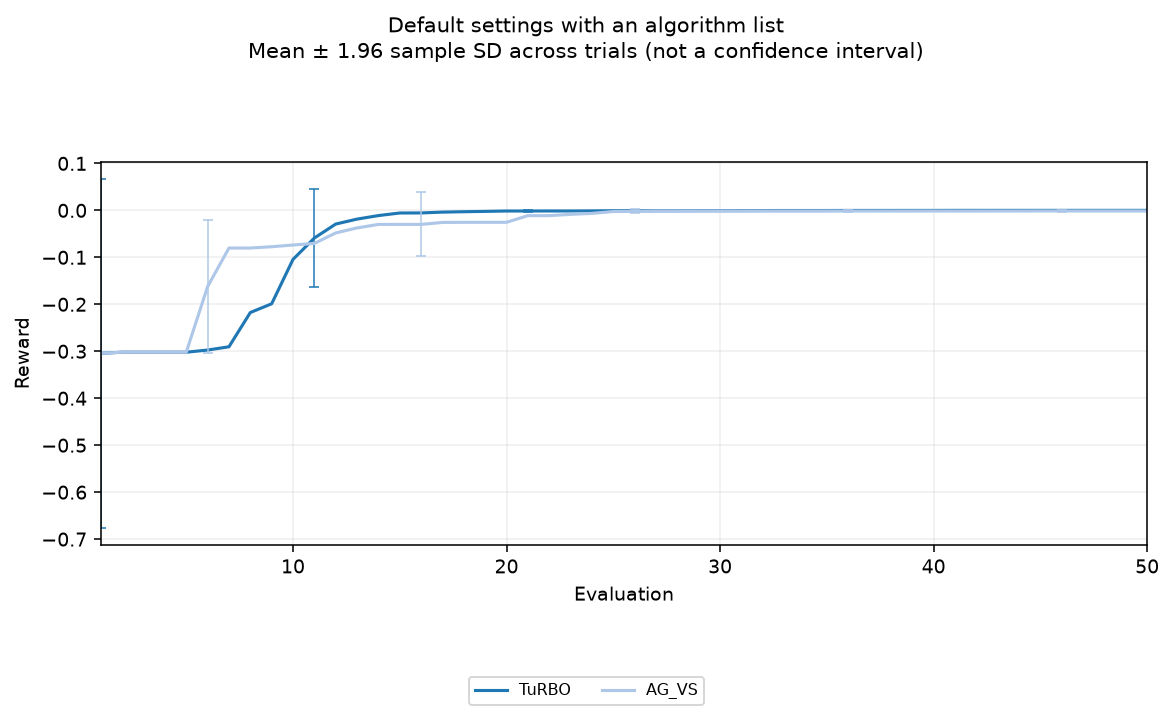
\includegraphics[width=\linewidth,height=.72\textheight,keepaspectratio]{figures/figure-11.png}

{\small\color{BayopyMuted}Captured figure 11 / settings defaults}

\end{center}

\end{minipage}\par\vspace{6pt}

\Needspace{6\baselineskip}
\phantomsection
\subsection*{Acquisition settings: UCB beta and EI offset}
\addcontentsline{toc}{subsection}{Acquisition settings: UCB beta and EI offset}

The three named configurations below all use TuRBO,\allowbreak{} with explicit EI/UCB extensions. UCB beta=9 has uncertainty multiplier 3; beta=3 has multiplier sqrt(3). \texttt{xi=\allowbreak{}0.01} changes EI's improvement threshold. These are comparisons of acquisition settings within the displayed trust-region implementation,\allowbreak{} not three separate algorithm families.



\BlockLabel{Editable Python / block 17}

\CodeFile{code/settings_acquisitions.py}

\BlockLabel{Captured terminal output}

\OutputFile{outputs/settings_acquisitions-01.txt}

\par\noindent\begin{minipage}{\linewidth}

\begin{center}

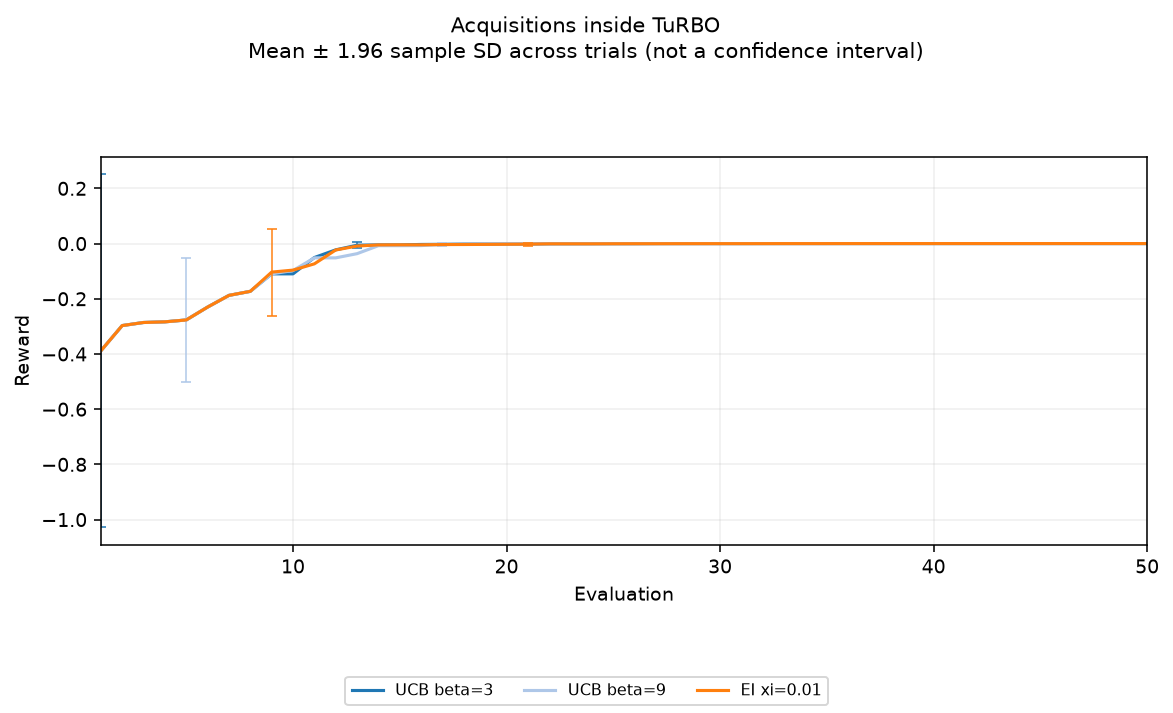
\includegraphics[width=\linewidth,height=.72\textheight,keepaspectratio]{figures/figure-12.png}

{\small\color{BayopyMuted}Captured figure 12 / settings acquisitions}

\end{center}

\end{minipage}\par\vspace{6pt}

\Needspace{6\baselineskip}
\phantomsection
\subsection*{GP kernels inside a contextual real-data experiment}
\addcontentsline{toc}{subsection}{GP kernels inside a contextual real-data experiment}

Here the kernel changes the surrogate used to choose measured Wine rows. We compare three CGP\_\allowbreak{}UCB configurations on the same dataset and seed,\allowbreak{} with the same fixed beta and optimizer budgets. The context kernel operates on one-hot cultivar,\allowbreak{} while the action kernel operates on the three scaled descriptors. These are optimization runs,\allowbreak{} not drawings of kernel functions.



\BlockLabel{Editable Python / block 18}

\CodeFile{code/settings_real_kernels.py}

\BlockLabel{Captured terminal output}

\OutputFile{outputs/settings_real_kernels-01.txt}

\par\noindent\begin{minipage}{\linewidth}

\begin{center}

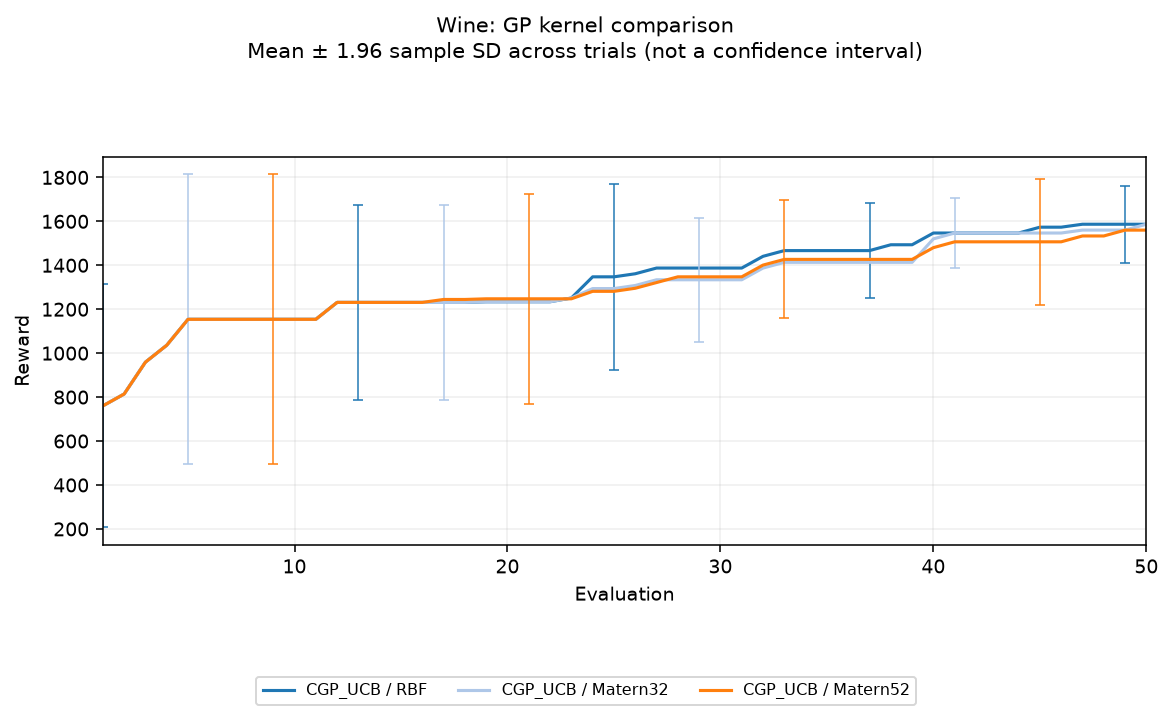
\includegraphics[width=\linewidth,height=.72\textheight,keepaspectratio]{figures/figure-13.png}

{\small\color{BayopyMuted}Captured figure 13 / settings real kernels}

\end{center}

\end{minipage}\par\vspace{6pt}

\Needspace{6\baselineskip}
\phantomsection
\subsection*{Sampling and batches}
\addcontentsline{toc}{subsection}{Sampling and batches}

Sampling overrides are attached to the experiment by algorithm label. The two TuRBO instances below compare Sobol and uniform sampling. Both request batches of 2,\allowbreak{} so 25 completed rounds consume 50 evaluations. \texttt{batch\_\allowbreak{}size=\allowbreak{}2} uses the method's independent batch behavior. For a supported joint Monte Carlo acquisition,\allowbreak{} use \texttt{batch\_\allowbreak{}size=\allowbreak{}None,\allowbreak{} q\_\allowbreak{}batch=\allowbreak{}2} instead; the third configuration demonstrates joint EI. The budget applies to actions,\allowbreak{} not rounds. Change a sampler only if that method supports the phase.



\BlockLabel{Editable Python / block 19}

\CodeFile{code/settings_sampling_batches.py}

\BlockLabel{Captured terminal output}

\OutputFile{outputs/settings_sampling_batches-01.txt}

\par\noindent\begin{minipage}{\linewidth}

\begin{center}

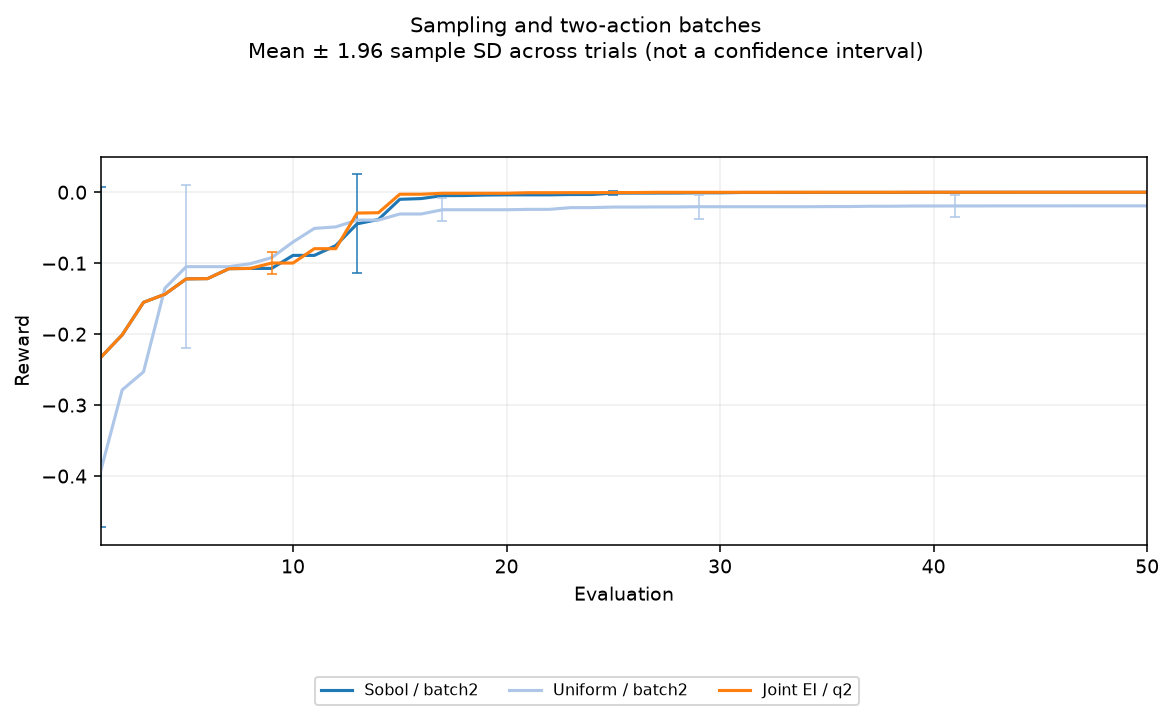
\includegraphics[width=\linewidth,height=.72\textheight,keepaspectratio]{figures/figure-14.png}

{\small\color{BayopyMuted}Captured figure 14 / settings sampling batches}

\end{center}

\end{minipage}\par\vspace{6pt}

\Needspace{6\baselineskip}
\phantomsection
\subsection*{Save,\allowbreak{} resume,\allowbreak{} and explicit display}
\addcontentsline{toc}{subsection}{Save,\allowbreak{} resume,\allowbreak{} and explicit display}

A single run writes into its chosen directory. A collection adds readable \texttt{algorithms/\allowbreak{}NN-label/\allowbreak{}} subdirectories and a combined \texttt{results.\allowbreak{}json}. Each method's settings,\allowbreak{} observations,\allowbreak{} diagnostics,\allowbreak{} and checkpoints remain separate. The runner saves final records even if a periodic \texttt{save\_\allowbreak{}every} checkpoint is not due. Repeated experiments add \texttt{trials/\allowbreak{}trial-001/\allowbreak{}} through \texttt{trials/\allowbreak{}trial-005/\allowbreak{}}; each trial contains its own method directories. Resuming uses total ceilings: resuming 10 evaluations with a cap of 50 adds at most 40 per trial. A fresh object must match the saved configuration.


\texttt{plot=\allowbreak{}False} disables the automatic progress plot. \texttt{plot=\allowbreak{}True,\allowbreak{} show=\allowbreak{}False} creates it without displaying it. \texttt{show=\allowbreak{}True} displays it on a capable backend. None of these settings change rewards or warning output. \texttt{bayopy.\allowbreak{}plot} controls title,\allowbreak{} axes,\allowbreak{} limits,\allowbreak{} legends,\allowbreak{} file saving,\allowbreak{} and display; assign its result to avoid notebook final-expression display when show=False. \texttt{bayopy.\allowbreak{}show} can display the retained plot explicitly.



\BlockLabel{Editable Python / block 20}

\CodeFile{code/settings_resume.py}

\BlockLabel{Captured terminal output}

\OutputFile{outputs/settings_resume-01.txt}

\par\noindent\begin{minipage}{\linewidth}

\begin{center}

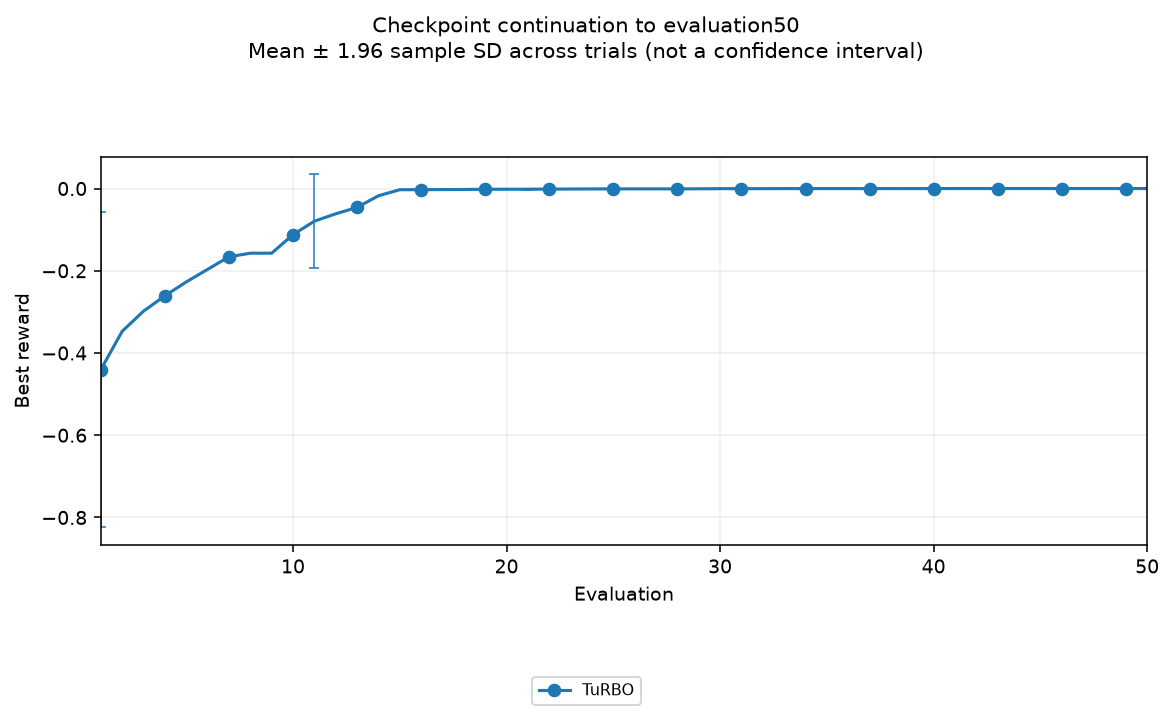
\includegraphics[width=\linewidth,height=.72\textheight,keepaspectratio]{figures/figure-15.png}

{\small\color{BayopyMuted}Captured figure 15 / settings resume}

\end{center}

\end{minipage}\par\vspace{6pt}

\clearpage
\phantomsection
\section*{Appendix A. Algorithm adaptations across environments}
\addcontentsline{toc}{section}{Appendix A. Algorithm adaptations across environments}

This appendix describes the current BayOPy implementation. An adaptation preserves the original environment,\allowbreak{} its evaluator,\allowbreak{} candidate restrictions,\allowbreak{} noise,\allowbreak{} and actual rewards. It supplies missing learner inputs or ignores unused metadata; it does not replace a distributional,\allowbreak{} contextual,\allowbreak{} or adversarial environment with a stochastic environment.


An algorithm outputs an action or evaluation query. The environment returns the scalar reward and feedback. Here,\allowbreak{} x denotes the selected action,\allowbreak{} x\_\allowbreak{}eval the actual evaluated location,\allowbreak{} c a context,\allowbreak{} C finite context support,\allowbreak{} and p reference probabilities over C. Information must be available at the correct time: a future sampled context must never be revealed before selection.


\Needspace{6\baselineskip}
\phantomsection
\subsection*{A.1. Stochastic algorithms}
\addcontentsline{toc}{subsection}{A.1. Stochastic algorithms}

The 14 stochastic-family algorithms are REMBO,\allowbreak{} HeSBO,\allowbreak{} ALEBO,\allowbreak{} ADD\_\allowbreak{}GP\_\allowbreak{}UCB,\allowbreak{} TuRBO,\allowbreak{} Dropout,\allowbreak{} MCTS\_\allowbreak{}VS,\allowbreak{} SAASBO,\allowbreak{} AG\_\allowbreak{}VS,\allowbreak{} LA\_\allowbreak{}MCTS,\allowbreak{} PG,\allowbreak{} EG,\allowbreak{} GS,\allowbreak{} and Satisficing\_\allowbreak{}TS. Their shared environmental inputs are the action domain or available candidates and previous actions and rewards. Their output is the next action,\allowbreak{} or a batch where supported. They do not require contexts or reference distributions to choose an action.


Their modeling requirements differ: REMBO,\allowbreak{} HeSBO,\allowbreak{} and ALEBO use low-dimensional embeddings; ADD\_\allowbreak{}GP\_\allowbreak{}UCB uses additive groups; TuRBO uses local trust regions; Dropout,\allowbreak{} MCTS\_\allowbreak{}VS,\allowbreak{} and AG\_\allowbreak{}VS select variables; LA\_\allowbreak{}MCTS partitions the domain; SAASBO uses a sparse-axis GP prior and posterior inference. PG,\allowbreak{} EG,\allowbreak{} GS,\allowbreak{} and Satisficing\_\allowbreak{}TS use their respective goodness,\allowbreak{} improvement,\allowbreak{} or posterior-sampling criteria. Embedding dimension,\allowbreak{} kernels,\allowbreak{} confidence settings,\allowbreak{} and thresholds remain algorithm choices,\allowbreak{} not environment observations.


\Needspace{6\baselineskip}
\phantomsection
\subsubsection*{A.1.1. Native stochastic environment}
\addcontentsline{toc}{subsubsection}{A.1.1. Native stochastic environment}

The algorithm selects x,\allowbreak{} the environment evaluates the stochastic objective,\allowbreak{} and the observed reward updates the learner. Normally x\_\allowbreak{}eval equals x. Compatibility still depends on each method's assumptions,\allowbreak{} such as low effective dimensionality for embedding algorithms; successful execution does not establish those assumptions.


\Needspace{6\baselineskip}
\phantomsection
\subsubsection*{A.1.2. Stochastic algorithms in an adversarial environment}
\addcontentsline{toc}{subsubsection}{A.1.2. Stochastic algorithms in an adversarial environment}

The learner selects an action with its ordinary policy. The real adversarial environment applies its perturbation or response and returns the actual reward. Unneeded attack metadata is ignored; the learner does not acquire an adversarial acquisition rule.


REMBO,\allowbreak{} HeSBO,\allowbreak{} and ALEBO specifically retain the nominal action's embedded coordinates and associate the resulting reward with those coordinates. They therefore learn the response obtained by submitting that action,\allowbreak{} including the attack's effect. A changing attack can make that response nonstationary. This is a warned extension,\allowbreak{} not a claim of adversarial robustness.


\Needspace{6\baselineskip}
\phantomsection
\subsubsection*{A.1.3. Stochastic algorithms in a distributional environment}
\addcontentsline{toc}{subsubsection}{A.1.3. Stochastic algorithms in a distributional environment}

The learner chooses x without conditioning on support C or probabilities p. The environment then samples its real context and evaluates the objective under that context. The learner consumes the actual reward. Public reference probabilities do not replace the environment's actual sampling mechanism.


With stationary sampling,\allowbreak{} the observations can support learning average performance over encountered contexts. These algorithms do not explicitly optimize a worst-case distributional objective. Changing distributions can make their observed response nonstationary.


\Needspace{6\baselineskip}
\phantomsection
\subsubsection*{A.1.4. Stochastic algorithms in a contextual environment}
\addcontentsline{toc}{subsubsection}{A.1.4. Stochastic algorithms in a contextual environment}

The environment reveals its current context,\allowbreak{} but the learner ignores it as a model input. It still honors the currently available actions,\allowbreak{} including context-dependent CSV candidate restrictions. The reward comes from the real contextual evaluator.


The same action can produce different rewards in different contexts. Ignoring context does not provide a context-dependent decision policy,\allowbreak{} nor does it permit selecting unavailable rows.


\Needspace{6\baselineskip}
\phantomsection
\subsubsection*{A.1.5. Finite real-data adaptation}
\addcontentsline{toc}{subsubsection}{A.1.5. Finite real-data adaptation}

All finite-data policies select existing available rows; missing rewards are not invented or interpolated. REMBO uses least-squares row compression,\allowbreak{} HeSBO uses signed bucket averages,\allowbreak{} and ALEBO uses its B projection. With the default finite\_\allowbreak{}candidate\_\allowbreak{}mode="project",\allowbreak{} each scores real candidate rows in compressed coordinates and returns the original row. This is a separately warned finite-candidate extension. The "exact" mode retains stricter embedding-geometry checks.


ADD\_\allowbreak{}GP\_\allowbreak{}UCB scores complete rows instead of combining unrelated group optima. TuRBO restricts rows to its trust region. Dropout,\allowbreak{} MCTS\_\allowbreak{}VS,\allowbreak{} and AG\_\allowbreak{}VS score complete candidates through selected coordinates. LA\_\allowbreak{}MCTS enforces its classifier path. SAASBO and the satisficing methods evaluate their criteria on the available candidates. The environment retains control of context availability,\allowbreak{} distributional reward coverage,\allowbreak{} and actual evaluations.


\Needspace{6\baselineskip}
\phantomsection
\subsection*{A.2. Adversarial and robust algorithms}
\addcontentsline{toc}{subsection}{A.2. Adversarial and robust algorithms}

BayOPy groups AdveRS and StableOPT in this family. AdveRS needs a feasible action domain and rewards at actual evaluated locations,\allowbreak{} with perturbation information when available. It outputs an action using its robust-satisficing criterion. Its hidden actual attack budget is not required as a learner input.


StableOPT needs a domain and a chosen robustness neighborhood. It selects a robust center using a worst-neighborhood upper-confidence criterion,\allowbreak{} then an evaluation query using a lower-confidence criterion within the neighborhood. Feedback supplies the actual evaluated location and reward. Robust optimization of a stochastic function is a native StableOPT use case: an external attacker is not required. Its robustness radius and metric define its optimization criterion and remain legitimate user settings.


\Needspace{6\baselineskip}
\phantomsection
\subsubsection*{A.2.1. Adversarial environment}
\addcontentsline{toc}{subsubsection}{A.2.1. Adversarial environment}

Environment-provided evaluated coordinates and perturbations take precedence. Both implementations train their GP at the location where the reward was actually observed. For StableOPT,\allowbreak{} an external attack is an additional extension because it can move the evaluation away from the query chosen by its robust procedure.


\Needspace{6\baselineskip}
\phantomsection
\subsubsection*{A.2.2. Adversarial/robust algorithms in a stochastic environment}
\addcontentsline{toc}{subsubsection}{A.2.2. Adversarial/robust algorithms in a stochastic environment}

For AdveRS,\allowbreak{} missing x\_\allowbreak{}eval defaults to x. Missing perturbation defaults to x\_\allowbreak{}eval minus x,\allowbreak{} which is zero when no attack or displacement is reported. Supplied displacement information is preserved. The source evaluates its original stochastic objective,\allowbreak{} while AdveRS retains its robust-satisficing criterion.


StableOPT can operate directly on the stochastic objective. Its chosen robustness neighborhood remains active even when the source applies no external attack. No attack does not mean a zero robustness radius.


\Needspace{6\baselineskip}
\phantomsection
\subsubsection*{A.2.3. Adversarial/robust algorithms in a distributional environment}
\addcontentsline{toc}{subsubsection}{A.2.3. Adversarial/robust algorithms in a distributional environment}

The learner selects an action or query,\allowbreak{} and the distributional source samples its context and returns the corresponding reward. These policies ignore reference probabilities and context as conditioning inputs. Actual evaluated coordinates are preserved; missing external-attack metadata uses the defaults above.


Their action-space robustness criterion is not a distributional robustness criterion. Variation caused by context remains part of their observed response. The run proceeds with a cross-environment diagnostic.


\Needspace{6\baselineskip}
\phantomsection
\subsubsection*{A.2.4. Adversarial/robust algorithms in a contextual environment}
\addcontentsline{toc}{subsubsection}{A.2.4. Adversarial/robust algorithms in a contextual environment}

The source retains its actual context and any context-dependent candidate restrictions. The algorithms select without conditioning their GP on that context and receive the true context-dependent reward. AdveRS defaults to zero external displacement when none is reported; StableOPT retains its selected robustness neighborhood.


Neither adaptation implements CGP\_\allowbreak{}UCB's contextual policy. In finite data,\allowbreak{} required neighborhood queries must exist as available rows. A fallback cannot manufacture missing evaluations.


\Needspace{6\baselineskip}
\phantomsection
\subsection*{A.3. Distributional algorithms}
\addcontentsline{toc}{subsection}{A.3. Distributional algorithms}

The native algorithms are DRBO and RoBOS. Both need public finite support C and reference probabilities p before selection,\allowbreak{} and the realized context and reward afterward. They output an action before the future context realization is known. DRBO additionally needs an ambiguity margin epsilon. RoBOS uses its aspiration-based formulation and does not require DRBO's ambiguity margin.


\Needspace{6\baselineskip}
\phantomsection
\subsubsection*{A.3.1. Native distributional environment}
\addcontentsline{toc}{subsubsection}{A.3.1. Native distributional environment}

The environment supplies support and reference information before selection and reveals the actual realization with the reward. The private sampling distribution remains private. Native support and its ordering stay fixed; references and DRBO's margin may vary between rounds. Algorithm configuration retains tunable kernels,\allowbreak{} confidence,\allowbreak{} divergence/solver choices,\allowbreak{} and aspiration where applicable.


\Needspace{6\baselineskip}
\phantomsection
\subsubsection*{A.3.2. Distributional algorithms in a stochastic environment}
\addcontentsline{toc}{subsubsection}{A.3.2. Distributional algorithms in a stochastic environment}

When all context and distribution inputs are absent,\allowbreak{} context defaults to a zero vector,\allowbreak{} support to the singleton containing that vector,\allowbreak{} probabilities to [1.0],\allowbreak{} and DRBO's ambiguity margin to 0. The source evaluates its original objective; the observation is recorded with the constant context.


The distributional calculation reduces to a singleton-context problem. It is executable but does not create meaningful uncertainty across multiple contexts.


\Needspace{6\baselineskip}
\phantomsection
\subsubsection*{A.3.3. Distributional algorithms in an adversarial environment}
\addcontentsline{toc}{subsubsection}{A.3.3. Distributional algorithms in an adversarial environment}

The same singleton defaults apply if no context or distribution information is provided. The actual adversarial source still applies its attack and returns the resulting reward and evaluated location.


A context-distribution fallback does not model the attacker. In particular,\allowbreak{} DRBO's ambiguity margin is not an action-perturbation budget. Execution continues as a warned extension without an adversarial robustness claim.


\Needspace{6\baselineskip}
\phantomsection
\subsubsection*{A.3.4. Distributional algorithms in a contextual environment}
\addcontentsline{toc}{subsubsection}{A.3.4. Distributional algorithms in a contextual environment}

If the source reveals c\_\allowbreak{}t but no distribution,\allowbreak{} the round's support becomes the singleton \{c\_\allowbreak{}t\},\allowbreak{} its reference probabilities are [1.0],\allowbreak{} and DRBO's margin defaults to 0. Selection uses this revealed context. The joint GP stores actual historical contexts and rewards.


The singleton integration support changes when the revealed context changes. Historical contexts are not overwritten. This is an explicitly warned extension of the native fixed-support distributional formulation.


For every adaptation,\allowbreak{} defaults apply independently: supplied support is retained,\allowbreak{} and supplied reference probabilities override fallback probabilities. When no reference is supplied,\allowbreak{} use a point mass on a provided current context when represented in support,\allowbreak{} otherwise uniform probabilities over known support when no current context is available. Malformed or incompatible supplied information is not silently repaired.


\Needspace{6\baselineskip}
\phantomsection
\subsection*{A.4. Contextual algorithms}
\addcontentsline{toc}{subsection}{A.4. Contextual algorithms}

CGP\_\allowbreak{}UCB is the native contextual algorithm. It needs the current context before selecting an action,\allowbreak{} the action domain or candidates,\allowbreak{} and previous observations. It models action-context pairs and outputs an action chosen for the decision context.


\Needspace{6\baselineskip}
\phantomsection
\subsubsection*{A.4.1. Native contextual environment}
\addcontentsline{toc}{subsubsection}{A.4.1. Native contextual environment}

The source reveals c\_\allowbreak{}t before selection. CGP\_\allowbreak{}UCB chooses an action using its joint GP and trains on the corresponding action-context observation after receiving the reward. Native feedback context must agree with the decision context.


\Needspace{6\baselineskip}
\phantomsection
\subsubsection*{A.4.2. CGP\_\allowbreak{}UCB in a stochastic environment}
\addcontentsline{toc}{subsubsection}{A.4.2. CGP\_\allowbreak{}UCB in a stochastic environment}

Missing context becomes an internal zero vector,\allowbreak{} used for both selection and observation. Its dimension follows public support or the context-kernel dimension when known,\allowbreak{} otherwise one. The source still evaluates its actual objective. A constant context supplies no changing contextual information for the learner to exploit.


\Needspace{6\baselineskip}
\phantomsection
\subsubsection*{A.4.3. CGP\_\allowbreak{}UCB in an adversarial environment}
\addcontentsline{toc}{subsubsection}{A.4.3. CGP\_\allowbreak{}UCB in an adversarial environment}

Missing context uses the same zero-vector default. The adversarial source still applies its attack,\allowbreak{} and its actual evaluated location and reward are retained. The learner uses the default context for the observation. This does not add an adversarially robust decision criterion; warnings identify the family mismatch and missing context.


\Needspace{6\baselineskip}
\phantomsection
\subsubsection*{A.4.4. CGP\_\allowbreak{}UCB in a distributional environment}
\addcontentsline{toc}{subsubsection}{A.4.4. CGP\_\allowbreak{}UCB in a distributional environment}

The actual future realization is unavailable before selection. The current automatic adaptation therefore selects using the zero-context default. After the source samples and evaluates,\allowbreak{} the learner trains using the actual context revealed with the reward. Decision context and training context can consequently differ in this extension.


The automatic adaptation does not use the distribution mean as the decision context. A separate explicit distribution\_\allowbreak{}mean\_\allowbreak{}context adapter is another modeling choice. Neither choice reproduces native contextual information timing; performance can suffer when the default decision context is unrepresentative.


\Needspace{6\baselineskip}
\phantomsection
\subsection*{A.5. Shared precedence,\allowbreak{} warnings,\allowbreak{} and limits}
\addcontentsline{toc}{subsection}{A.5. Shared precedence,\allowbreak{} warnings,\allowbreak{} and limits}

Environment-provided values override internal defaults independently for each field. Extra metadata is ignored by algorithms that do not need it,\allowbreak{} but can still influence the source's actual reward. Missing inputs receive defaults only when those defaults make execution well-defined. Standalone historical initialization likewise retains supplied contexts and warns when substituting missing historical values.


Context observations,\allowbreak{} support,\allowbreak{} reference distributions,\allowbreak{} and actual external perturbations belong to the environment. They are not ordinary AlgorithmConfig parameters. Scientific choices such as kernels,\allowbreak{} confidence levels,\allowbreak{} aspiration,\allowbreak{} embedding dimensions,\allowbreak{} and StableOPT's chosen robustness criterion remain tunable.


Cross-family diagnostics identify the native-family mismatch and any expected information that was missing,\allowbreak{} together with the fallback actually used. Successful execution does not transfer published guarantees. Invalid supplied values,\allowbreak{} incompatible model dimensions,\allowbreak{} and impossible candidate constraints remain errors or explicit stopping conditions. Finite exhaustion stops cleanly; an insufficient atomic batch is not completed with fabricated rows.


This appendix documents the implementation and its limitations; it adds no new experimental measurements. The earlier five-trial results and their recorded numerical diagnostics remain unchanged.



\end{document}
